%\documentclass[review]{elsarticle}
\documentclass[5p,times]{elsarticle}
\usepackage{lineno,hyperref}
\usepackage{amssymb}
\usepackage{stfloats}
\modulolinenumbers[5]
\usepackage{lipsum}
\usepackage{pifont}
\usepackage{graphicx}
\usepackage{subfigure}
\usepackage{amsmath}
\usepackage[ruled,linesnumbered]{algorithm2e}
\usepackage{ulem}

\journal{Journal of \LaTeX\ Templates}

%%%%%%%%%%%%%%%%%%%%%%%
%% Elsevier bibliography styles
%%%%%%%%%%%%%%%%%%%%%%%
%% To change the style, put a % in front of the second line of the current style and
%% remove the % from the second line of the style you would like to use.
%%%%%%%%%%%%%%%%%%%%%%%

%% Numbered
%\bibliographystyle{model1-num-names}

%% Numbered without titles
%\bibliographystyle{model1a-num-names}

%% Harvard
%\bibliographystyle{model2-names.bst}\biboptions{authoryear}

%% Vancouver numbered
%\usepackage{numcompress}\bibliographystyle{model3-num-names}

%% Vancouver name/year
%\usepackage{numcompress}\bibliographystyle{model4-names}\biboptions{authoryear}

%% APA style
%\bibliographystyle{model5-names}\biboptions{authoryear}

%% AMA style
%\usepackage{numcompress}\bibliographystyle{model6-num-names}

%% `Elsevier LaTeX' style
\bibliographystyle{elsarticle-num}
%%%%%%%%%%%%%%%%%%%%%%%

\begin{document}

\begin{frontmatter}

\title{GLEX-Alltoall: Overlapped Numa-aware Multi-leader Multi-port alltoall algorithm on Multi-core Supercomputer}

%% Group authors per affiliation:
\author{Jintao Peng\fnref{pjtnote}}
\author{Jie Liu\fnref{ljnote}\corref{mycorrespondingauthor}}
\author{Min Xie\fnref{xmnote}}

\address{Changsha, China}
\fntext[pjtnote]{JintaoPengCS@gmail.com}
\cortext[mycorrespondingauthor]{Corresponding author}
\fntext[ljnote]{liujie@nudt.edu.cn}
\fntext[xmnote]{xiemin@nudt.edu.cn}



\begin{abstract}
		All-to-all communication is commonly used in parallel applications like FFT. 
		In mordern supercomputers, there are multiple cores in a node.
		To optimize all-to-all communication, a typical way is gather-scatter-based alltoall which aggregate messages on each pair of nodes.
		Multiple cores, NUMAs and network endpoints bring much parallelism. 
		However, there is no method which makes uses these parallelism to improve the all-to-all communication. 
		In this paper, we introduce Overlapped Numa-aware Multi-leader Multi-port alltoall (ONMPML) collectives which explore the parallelism on network, CPU cores and overlap the intra- and inter-node communication. 
		The results show that, compared to MPI, our library achieves up to 20x speedup. 
		For application, our method achieves up to 17x speedup on peak performance for 16384 cores.
\end{abstract}

 \begin{keyword}
 Collective Communication \sep Multi-core processor \sep MPI all-to-all \sep RDMA \sep Shared Heap
\MSC[2010] 00-01\sep  99-00
\end{keyword}

\end{frontmatter}

\linenumbers

\section{Introduction}
%对于很多并行应用而言,全局的通信往往成为限制其扩展性的关键点。
%聚合通信作为普遍使用的全局通信,在各种应用种广泛使用。
%all-to-all通信作为聚合通信之一,在FFT和图计算应用中有重要应用。
%然而all-to-all通信在任意两个进程之间都需要发消息。每次并行规模翻倍,all-to-all通信量翻4倍。
%另一方面,网络吞吐率和节点数量的增加则是线性增长。
%这给大规模all-to-all通信带来巨大的挑战。

%典型的方法是在节点内进行聚合消息然后在节点间传输数据。
%简单的说就是将MPI_alltoall替换为n次gather+节点间alltoall+n次scatter。
%该方法对于小消息非常有效。
%通过这种方法消息数量降低节点内进程数量的平方倍。
%在当前超级计算机结构下,有4种并行性有助于优化该节点感知的all-to-all的通信性能:
%多个网络端口使得网卡可以同时处理多个通信请求。
%多个内存控制器/NUMA/内存通道,带来的访存并行性。
%多核心带来的通信请求构造数据Gather和Scatter的并行性。
%节点内和节点间数据传输的并行性。
%但是据我们所知,没有一种节点感知的all-to-all方法充分发掘了这四种并行性。

%在节点内,优化节点感知的all-to-all通信算法在节点内的典型方法有共享内存。
%该方法能够使得节点内通信绕过网卡进行。
%此外,内核辅助的“零拷贝”技术以及共享堆的也是常见的方法。
%这些方法能够降低一次点内的内存拷贝次数。
%同时也有一些方法考虑到了NUMA/UMA中的cache利用效率的问题。
%但是这些方法并没有考虑到随着超级计算机的发展,节点间通信并不会比节点内通信慢太多。
%现代超级计算机普遍装备着多核心,多numa的处理器。
%典型的方法通常没有将这其中的并行性发掘出来。

%本文提出了一种多leader的节点感知all-to-all通信库。
%利用多个核心进行本地转置,发掘多核并行。
%使用多核CPU核心同时进行Gather和Scatter操作,发掘多NUMA并行访存。
%利用多个网络端口同时进行消息传输,发掘网络并行行。
%将节点内和节点间数据传输重叠起来,提升大消息通信性能。
%该通信库在节点内使用共享堆作为Gather和Scatter操作的基础。
%在节点间使用RDMA进行网络通信。
%实验表明,对于16384个进程,我们的通信库对比MPI可以实现最大10X的性能提升。从小消息到大消息平均可提升4.16倍。

Many parallel applications may suffer from global communication.
Especially for communication-intensive applications, their time-to-solution and scalablily may be affected by global communication. 
Message Passing Interface (MPI) provides a set of commonly used collective communication.
MPI\_Alltoall is one of the collective communication where each process will send a different message to all processes.
It is broadly used in some parallel applications like Fast Fourier Transform (FFT) \cite{mehta2021parallel} and some graph algorithms like MapReduce \cite{plimpton2011mapreduce} and Breadth-first search (BFS) \cite{ueno2012highly}.
However, each time we double the processes, the communication workload of all-to-all is quadrupled.
On mordern supercomputers, network throughput has a linear relationship with the number of nodes.
This brings great challenges to design large-scale all-to-all collectives.

For multiple-core supercomputers, an effective way is node-aware all-to-all method \cite{sistare1999optimization}.
A p (p=N times M, M is \#processes on a node) processes all-to-all is replaeced by a N node inter-node all-to-all. Which is: N-1 times intra-node gather + local transpose + inter-node transpose + N-1 times intra-node gather.
This method is very effective for small messages.
Because, compared to original method, a node-aware all-to-all reduce the number of inter-node messages from $(M^N)^2$ to $N^2$ times.
The size of the message is increased by $M^2$ times, which can effective use of the network bandwidth.
On the current supercomputer, there may be 20-64 CPU cores in a node.
The single message size can be scaled 400-4096 times.
In production environment, node-aware all-to-all may more efficient than Bruck's algorithm.


However, the gathering/scattering overhead on node-aware all-to-all make it hard to be scaled to larger messages.
Multiple CPU cores, NUMA and network endpoints brings 4 kinds of parallism to optimize a node-aware all-to-all method:
\begin{enumerate}[(1)]
\item Multiple network endpoints can simultaneously process multiple communication requests.
\item Processes in different NUMA can simultaneously access it local memory without contention.
\item Multiple processes can simultaneously gather/scatter data and compose communication requests.
\item Inter-node communication can be overlapped with intra-node communication.
\end{enumerate}
As we known, no methods combine these parallism togather to improve a node-aware all-to-all collective communication. 

% A typical intra-node communication is based on shared memory.
% Processes create a shared memory at initialization stage, the data is fistly copied from senders buffer into the shared memory buffer, then copied out to the receivers buffer.
% Two data copy needed to transer a intra-node message.
% To reduce the memory copy times, kernel-assisted communication, shared heaps, and thread-based MPI are proposed.

In this paper, we proposed Overlapped NUMA-aware Multi-port Multi-leader (ONMPML) method to scale the node-aware all-to-all collective.
ONMPML using multiple leaders on different NUMA to gather/scatter data, compose communication requests, and transpose local matrix and open the different network endpoints to do inter-node all-to-all.
ONMPML explore the parallelism existing in mordern multi-core processor with NUMA memory architecture and multi-port network.
For intra-node gather/sactter, we implemented a shared-heap-based remote accessible memory to support multiple leader to gather/scatter simutaneously.
Inter-node communication is implemented on Remote Direct Memory Access (RDMA) which provide high throughput and low latency.
The results show that, compared to MPI\_alltoall, our implementation achieves up to 18x speedup and 4x speedup on average. 
\section{Related Work}

Bruck algorithm \cite{bruck1997efficient} is commonly used for small message all-to-all. For mid size messages, isend-irecv algorithm is used. Linear shift exchange \cite{ranka1994static}, pairwise exchange\cite{thakur2005optimization} apply to large messages.

When considering the multi-core processors:  
Cache-oblivious MPI all-to-all (SH-NUMA-CO) based on morton order is proposed to minimize the cache miss rate \cite{li2017cache}.
For Infiniband on multi-core systems, a non-leader all-to-all collective (SA-orig) which based on shared memory aggregation techniques is proposed in \cite{kumar2008scaling}.
For multi-rail QsNet SMP clusters, a shared memory and RDMA based all-to-all collectives (elan\_alltoall) is proposed in \cite{qian2008efficient}.
For Intel Many Integrated Core (MIC) architecture,  the re-routing scheme based all-to-all collective (PAIRWISE-SLR/BRUCK-SLR) is proposed in \cite{venkatesh2014high}. 
As these works are all support leader-based aggreagation. 
Table \ref{relatedworkcompare} shows the overall design-space comparation between these methods and our method.

%我们用一个表格来展示这些方法和我们的方法的区别。

\begin{table*}[t]
    \caption{Overall design-space for all-to-all collective on mulit-core processers}\label{relatedworkcompare}
    \begin{tabular}{|l|c|c|c|c|c|}
        \hline
        Approach/Metric                  & \multicolumn{1}{l|}{SH-NUMA-CO} & \multicolumn{1}{l|}{SA-orig} & \multicolumn{1}{l|}{elan\_alltoall} & \multicolumn{1}{l|}{\begin{tabular}[c]{@{}l@{}}PAIRWISE-SLR\\ and BRUCK-SLR\end{tabular}} & \multicolumn{1}{l|}{\begin{tabular}[c]{@{}l@{}}ONMPML\\ (ours)\end{tabular}} \\ \hline
        inter-node implementation        & MVAPICH2                        & MVAPICH                      & RDMA                                & MPI-P2P                                                                                   & RDMA                                                                                             \\ \hline
        intra-node implementation        & Shared Heap                     & Shared Memory                & Shared Memory                       & MPI-P2P                                                                                   & Shared Heap                                                                                             \\ \hline
        Leader-based aggregation support & \ding{52}                        &\ding{52}                     &\ding{52}                            &\ding{52}                                                                                   &\ding{52}                                                                                                  \\ \hline
        Multi-leader support             &\ding{54}                        &\ding{52}                     &\ding{54}                            &\ding{54}                                                                                  &\ding{52}                                                                                                  \\ \hline
        NUMA-aware                       &\ding{52}                        &\ding{54}                     &\ding{54}                            &\ding{54}                                                                                  &\ding{52}                                                                                                  \\ \hline
        Multiple network endpoints       &\ding{54}                        &\ding{52}                     &\ding{52}                            &\ding{54}                                                                                  &\ding{52}                                                                                                  \\ \hline
        Overlapping Inter/intra-node     &\ding{52}                        &\ding{54}                     &\ding{54}                            &\ding{52}                                                                                  &\ding{52}                                                                                                  \\ \hline
        \end{tabular}
\end{table*}

Besides, to improve the intra-node communication, several kernel-assistant techniques have been proposed for multi-core processor ( LIMIC \cite{jin2007lightweight}, KNEM \cite{goglin2013knem}, XPMEM).
Compared to shared memory, these method works well for large message intra-node communication.
Because they avoid one memory copy overhead.
Shared heap \cite{li2014improved} has the same performance with these kernel-assistant techniques.
Shared heap do not need extra kernel module.

When considering the network topology: A bandwidth-optimal all-to-all exchange is proposed for fat-tree network \cite{prisacari2013bandwidth}. 
For torus network, a large scale all-to-all is proposed for Blue Gene/L Supercomputer \cite{kumar2008optimization}.  
A optimal schedule for all-to-all personalized communication is proposed for multiprocessor systems \cite{saha2019optimal}. 
For Infiniband clusters, their is a topology aware all-to-all scheduler which lower the contention by adding extra communication steps \cite{subramoni2014designing}.
A L-level hierarchy method which based on mapping of intensively communicating processes into the same computer nodes is proposed in \cite{kurnosov2016dynamic}. 
A method which considering dynamic performance model of the network is proposed at \cite{cui2020communication}.



\section {Experimental Platforms}
The methods in this paper are validated on two different systems:
\begin{enumerate}[(1)]
\item HPC-A: Matrix-2000+ CPU on each node, Tianhe series network.
\item HPC-B: E5-2692 v2 CPU * 2 on each node, Tianhe series network. 
\end{enumerate}
The memory bandwidth test (Stream) and network bandwidth test results are shown in the Table \ref{Memorybandwidth}.
\begin{table*}[]
    \caption{Memory Bandwidth (tested on Stream) and Point-to-Point Bandwidth (tested on RDMA) of Experimental Platforms}\label{Memorybandwidth}
\begin{tabular}{|l|c|c|c|c|c|c|c|}
\hline
\begin{tabular}[c]{@{}l@{}}Bandwidth tests \\ (MB/s)\end{tabular} & \begin{tabular}[c]{@{}c@{}}Copy\\ (Single-thread)\end{tabular} & \begin{tabular}[c]{@{}c@{}}Copy\\ (Multi-threads)\end{tabular} & \multicolumn{1}{l|}{\begin{tabular}[c]{@{}l@{}}NUMA \\ Count\end{tabular}} & \multicolumn{1}{l|}{\begin{tabular}[c]{@{}l@{}}loopback \\ banwdith\end{tabular}} & \multicolumn{1}{l|}{\begin{tabular}[c]{@{}l@{}}bi-loopback \\ banwdith\end{tabular}} & \multicolumn{1}{l|}{\begin{tabular}[c]{@{}l@{}}two node p2p \\ banwdith\end{tabular}} & \multicolumn{1}{l|}{\begin{tabular}[c]{@{}l@{}}two node bip2p \\ banwdith\end{tabular}} \\ \hline
HPC-A (32 cores)                                                      & 6481                                                           & 21351                                                          & 4                                                                          & 1366                          & 1368                             & 1181                              & 1336                                \\ \hline
HPC-B (24 cores)                                                      & 11280                                                          & 46252                                                          & 2                                                                          & 11530                         & 11568                            & 7089                              & 11629                               \\ \hline
\end{tabular}
\end{table*}
In table \ref{Memorybandwidth}, copy bandwidth is tested by STREAM. Loopback bandwidth means where sending process and receiving process is placed on a same node. Bi-loopback bandwidth is the bidirectional bandwidth of two processes on a same node.
\section {Motivation}

Node-aware all-to-all is a traditional method to optimize small message all-to-all.
Node-aware all-to-all will aggregate messages between each pair of node to reduce message number.

As shown in Figure ~\ref{Node-aware-alltoall}.
\begin{figure}[!htb]
  \centering
    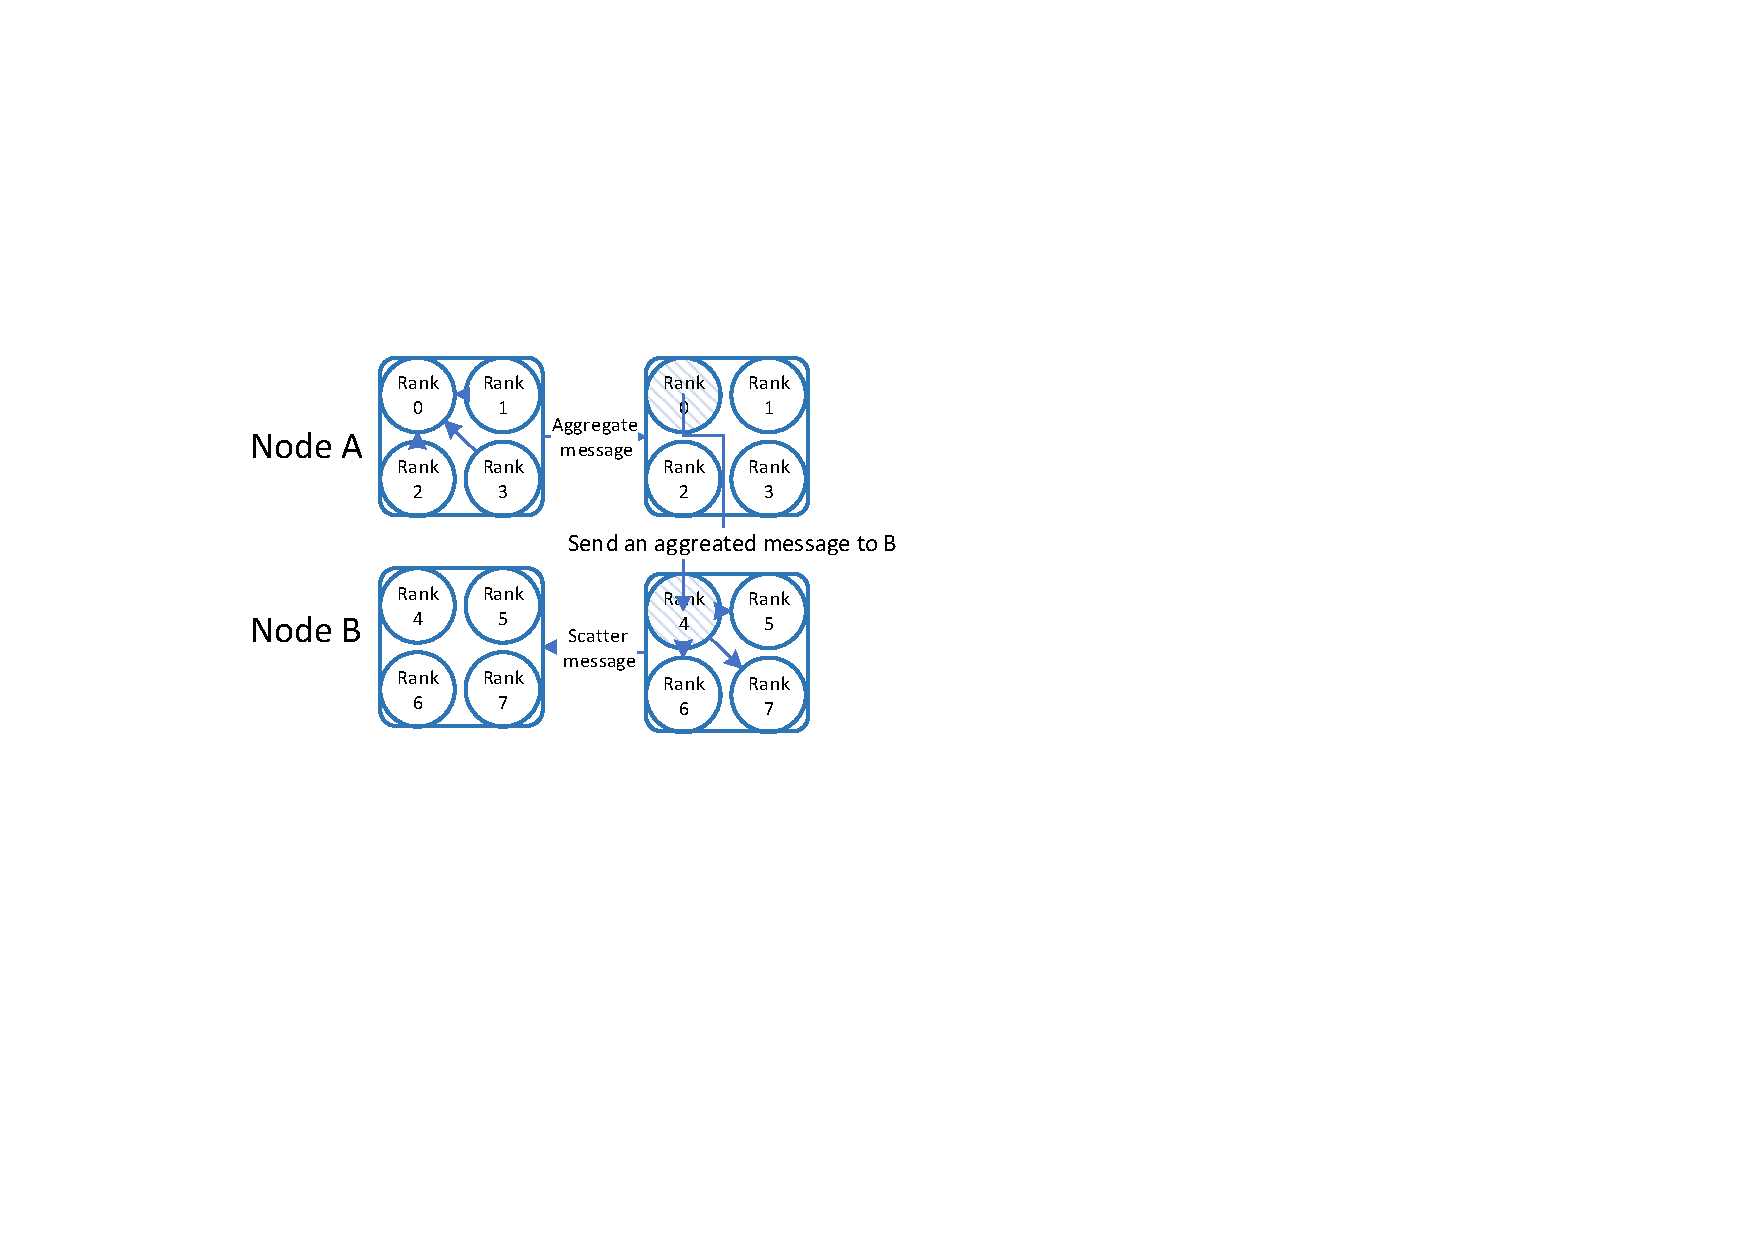
\includegraphics[width=0.49\textwidth]{./Figures/Node-aware-alltoall.pdf}
  \caption{Multi-leader gahtering/scattering throughput based on MPI-RMA, Leader Number $\in$ [1,2,4,8]}
	\label{Node-aware-alltoall}
	\vspace{0.2in}
\end{figure}

It include four steps: intra-node gather, local transpose, inter-node all-to-all, intra-node scatter.
For a 32/64 cores CPU, each inter-node message in node-aware method will be 1024/4096 times larger than direct method.
After aggreatation, the small messages become large messages and message number is reduced.
However, when message getting larger, gatering, transpose, and scattering overhead increase with the message size.
It limit the application scope of node-aware all-to-all.

With the increase in the number of processor cores, multiple CPU cores, NUMA, network endpoints and inter-/intra-node overlapping brings huge parallelism.
We notice that all traditional method do not take advantage of this parallelism to solve the problem.
As the single-core memory access bandwidth may not faster than the network bandwidth.
Using a single core to gather, scatter, and transpose data, and initialize communication request may causing communication hotspot on a CPU core.

Multi-leader can get faster message aggregation throughput than one-leader gathering/scattering.
Results of figure \ref{multileader-gather} show the multi-leader gathering/scattering throughput compared to one-leader.
\begin{figure*}[!htb]
  \centering
    \subfigure[HPC-A]{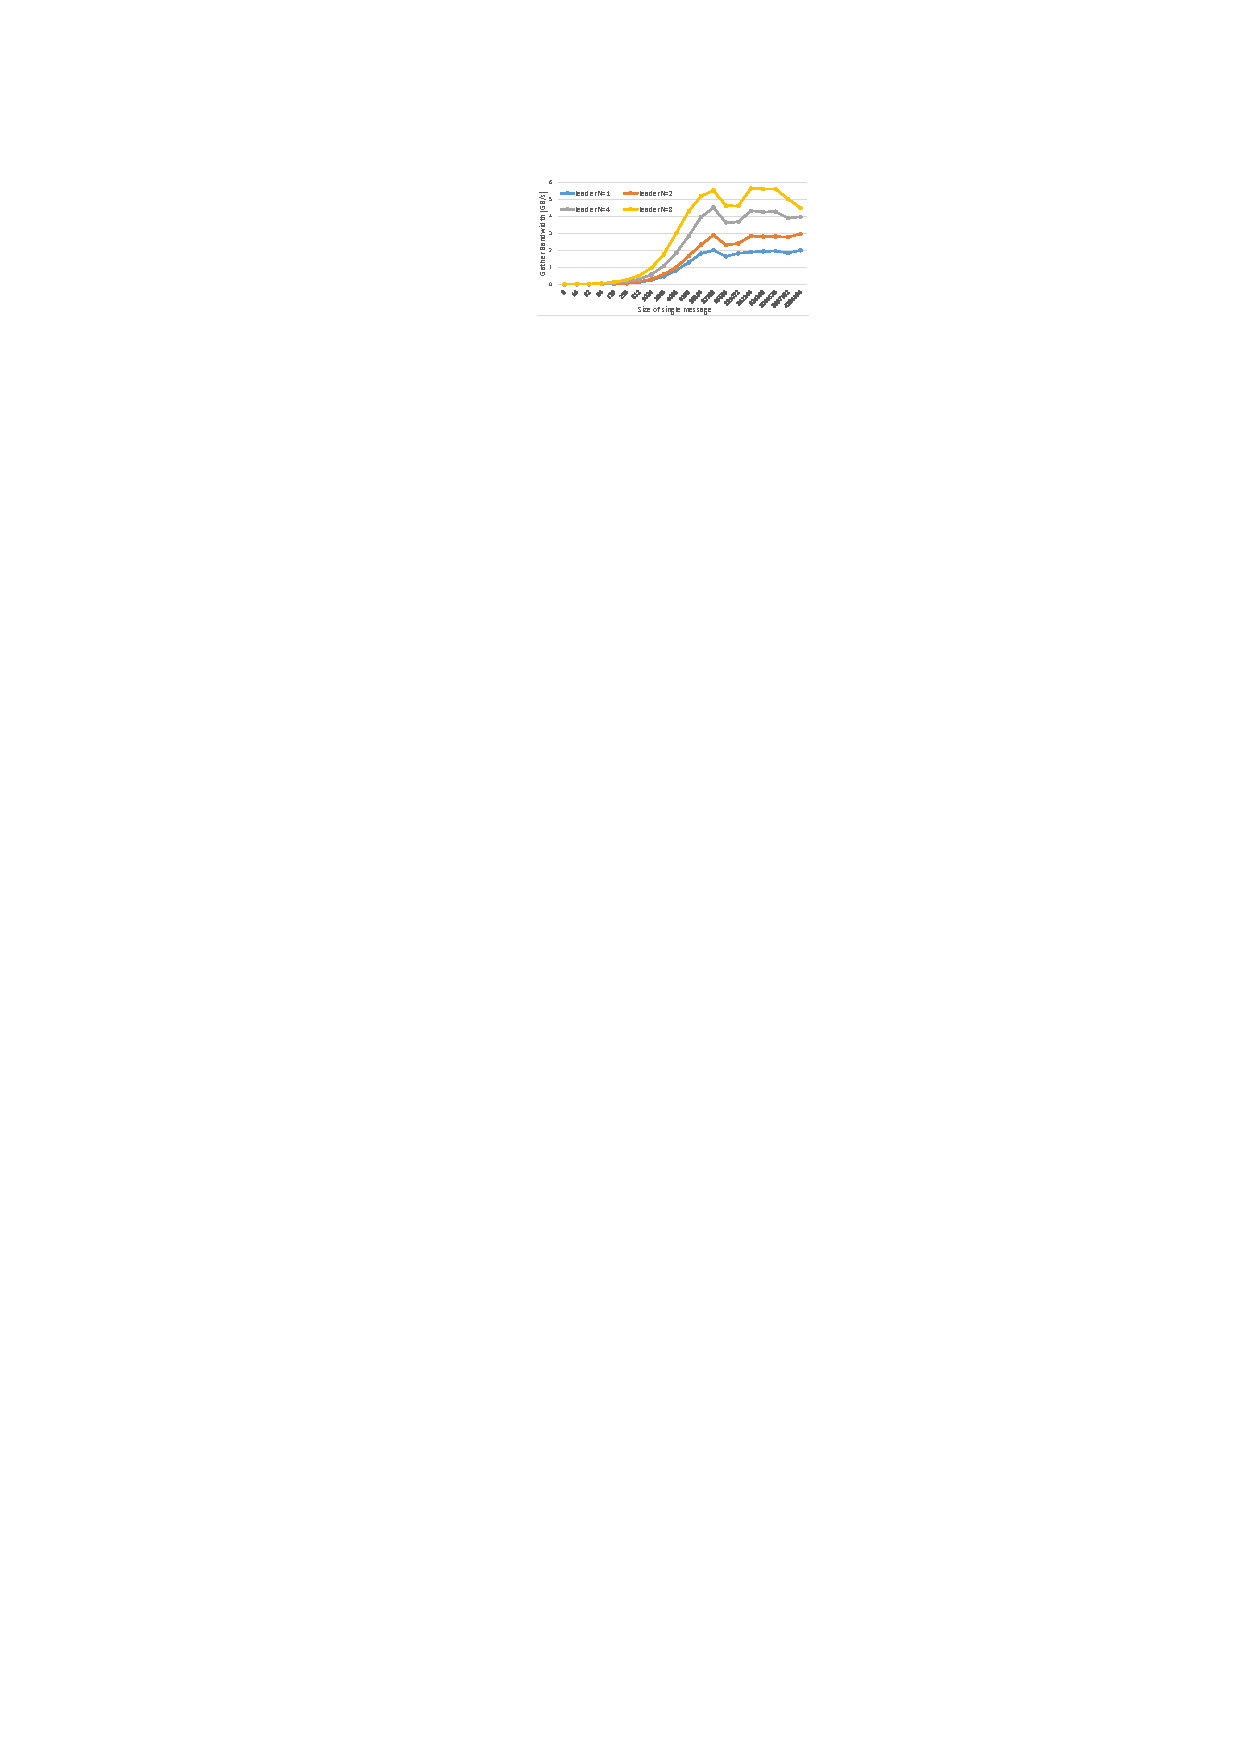
\includegraphics[width=0.49\textwidth]{./Figures/hpca/HPC-multi-leader-gather.pdf}}
	\subfigure[HPC-B]{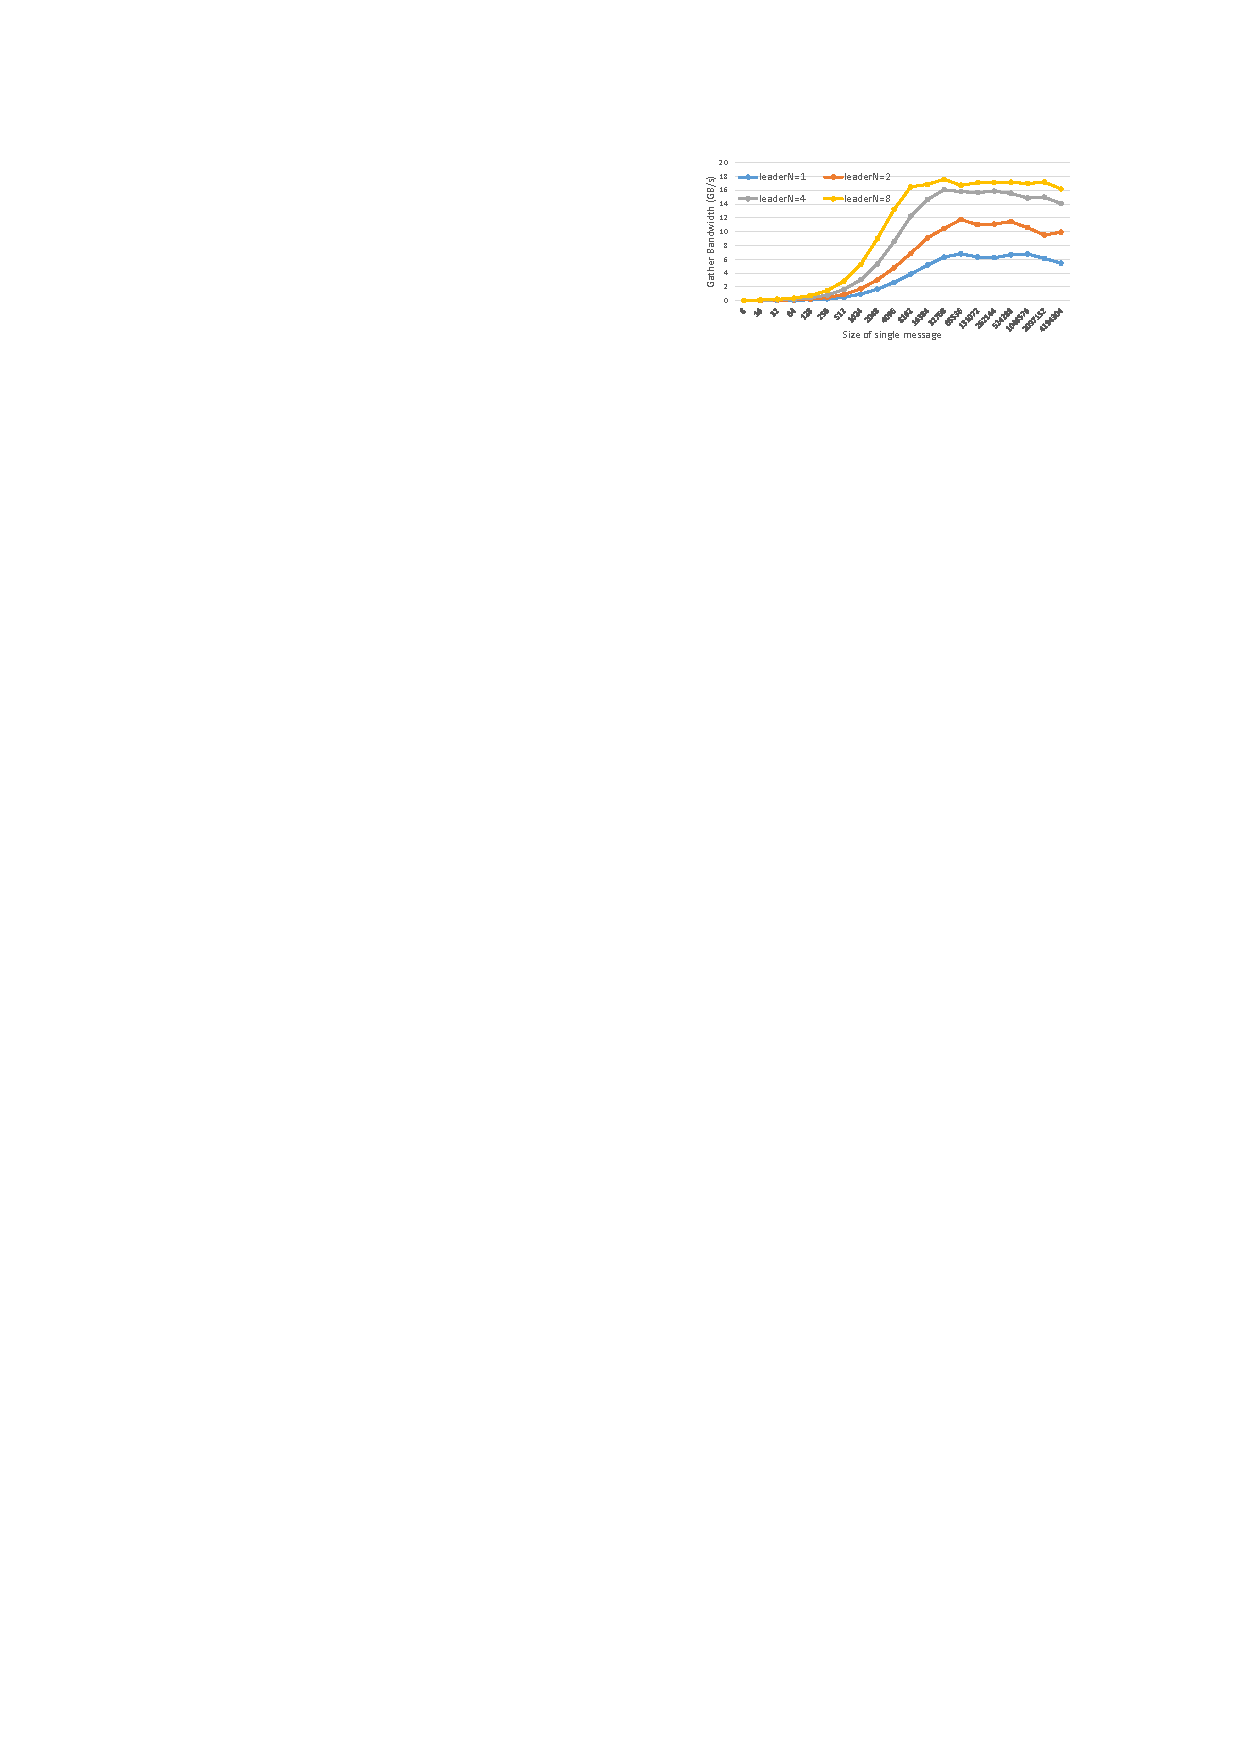
\includegraphics[width=0.49\textwidth]{./Figures/hpcd/HPC-multi-leader-gather.pdf}}
  \caption{Multi-leader gahtering/scattering throughput based on MPI-RMA, Leader Number $\in$ [1,2,4,8]}
	\label{multileader-gather}
	\vspace{0.2in}
\end{figure*}
Notice the result of HPC-B, its one-leader gathering/scattering bandwidth is about 6 GB/s, while it p2p bandwidth is 7.089 GB/s.
As a node-aware all-to-all includes: intra-node gather, inter-node all-to-all, intra-node scatter steps.
The overhead to aggregate M gigabyte messages is about M/6 second.
The overhead to send it to another node is about M/7 second.
The overhead to scatter it on is about M/6 second.
In this case, intra-node communication become  bottelneck of node-aware all-to-all.
Using multiple leaders can improve the gathering and scattering thoughput on a node.

With non-uniform memory access (NUMA) systems has emerged, a CPU is composed with multi-socket. 
When different core try to access a same NUMA, its local memory bandwidth is shared between multiple cores.
For a Multi-leader gathering/scattering on these processors, NUMA architecture has performance effect on gathering/scattering performance. 
Putting multiple leader on the same NUMA or lets leaders uniform distributed on the CPU may have significant performance difference.
We bind each processes to corresponding core and compared the NUMA-aware and test the NUMA-aware multi-leader gahtering/scattering  Vs multi-leader gahtering/scattering.
The performance improvements are shown in Figure \ref{UMA-aware-multi-leader}.
Because the CPU has multiple memory access units for different NUMAs.
\begin{figure*}[!htb]
  \centering
    \subfigure[HPC-A 4 NUMAs in a node]{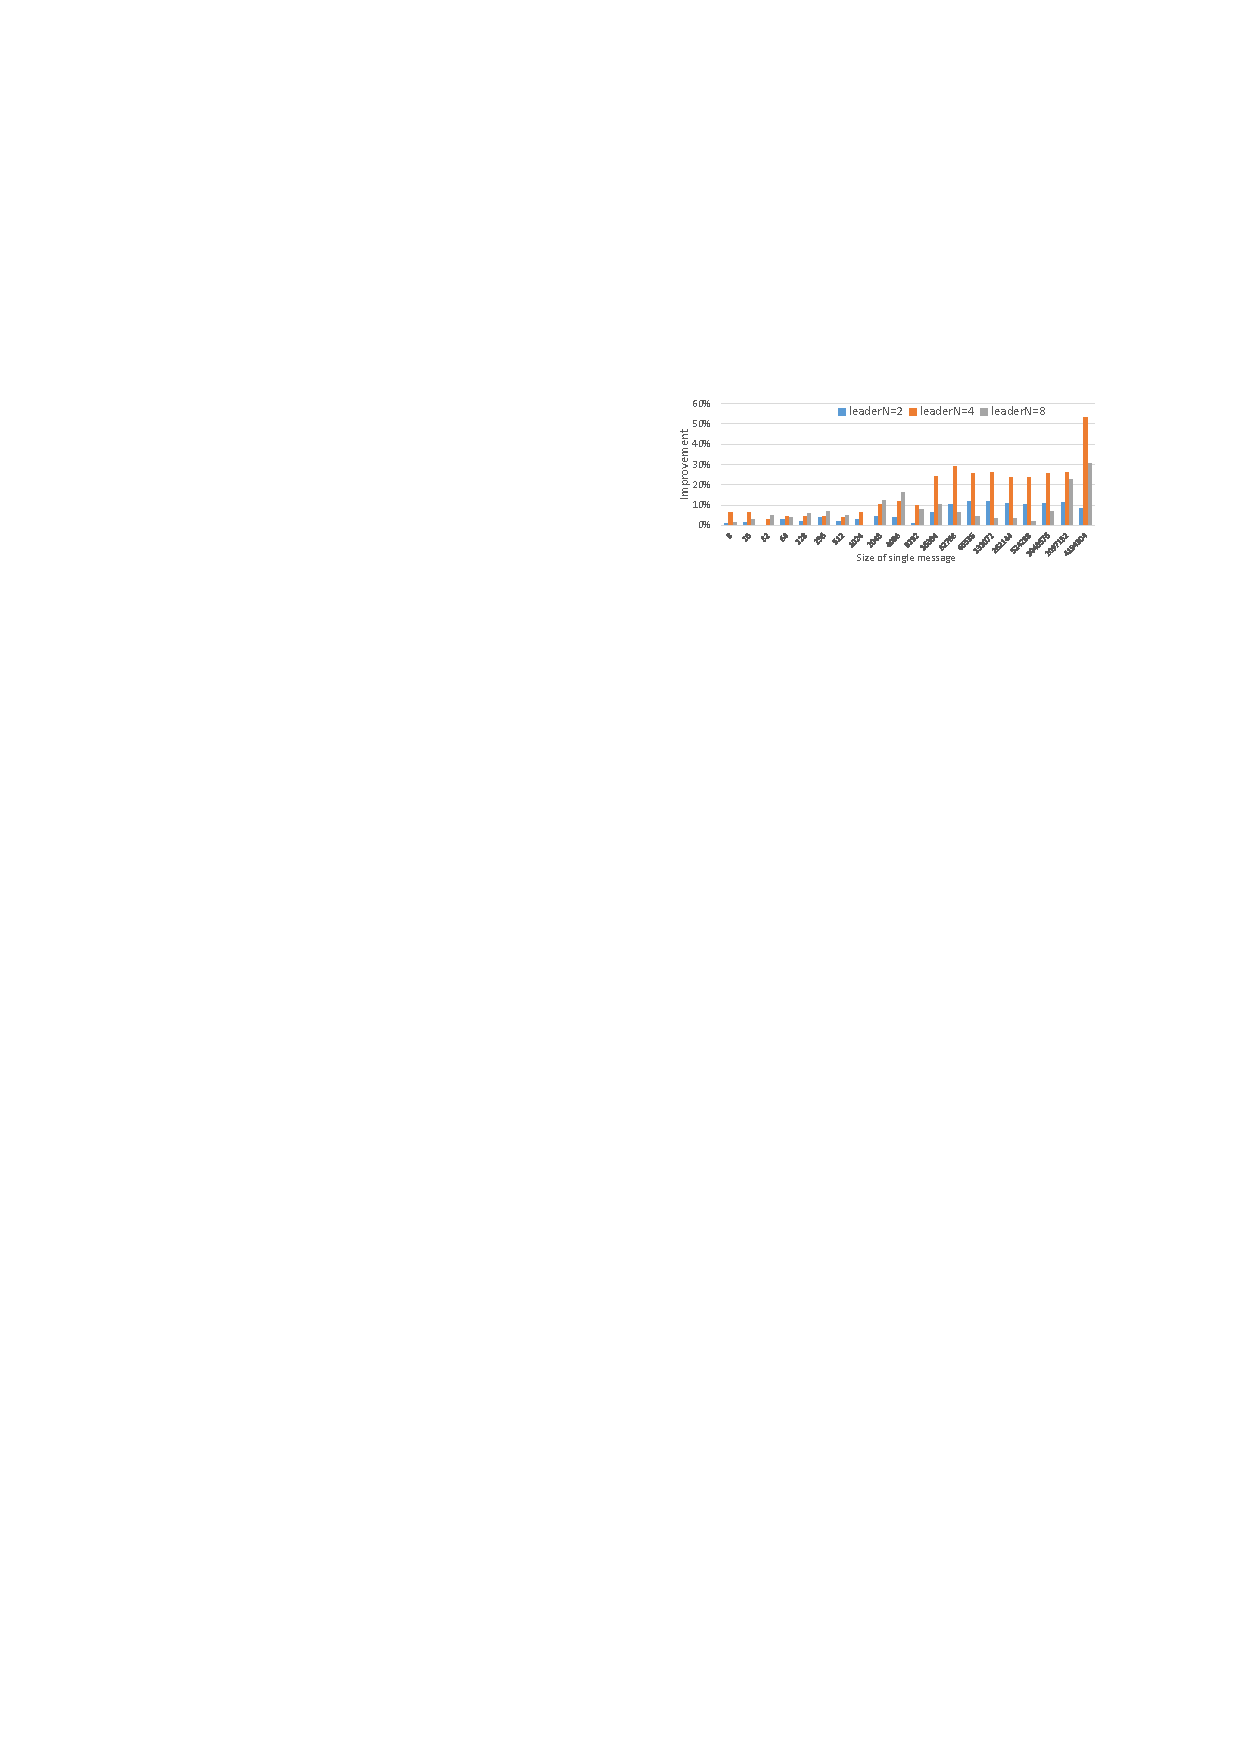
\includegraphics[width=0.49\textwidth]{./Figures/hpca/NUMA-aware-gather-scatter.pdf}}
	\subfigure[HPC-B 2 NUMAs in a node]{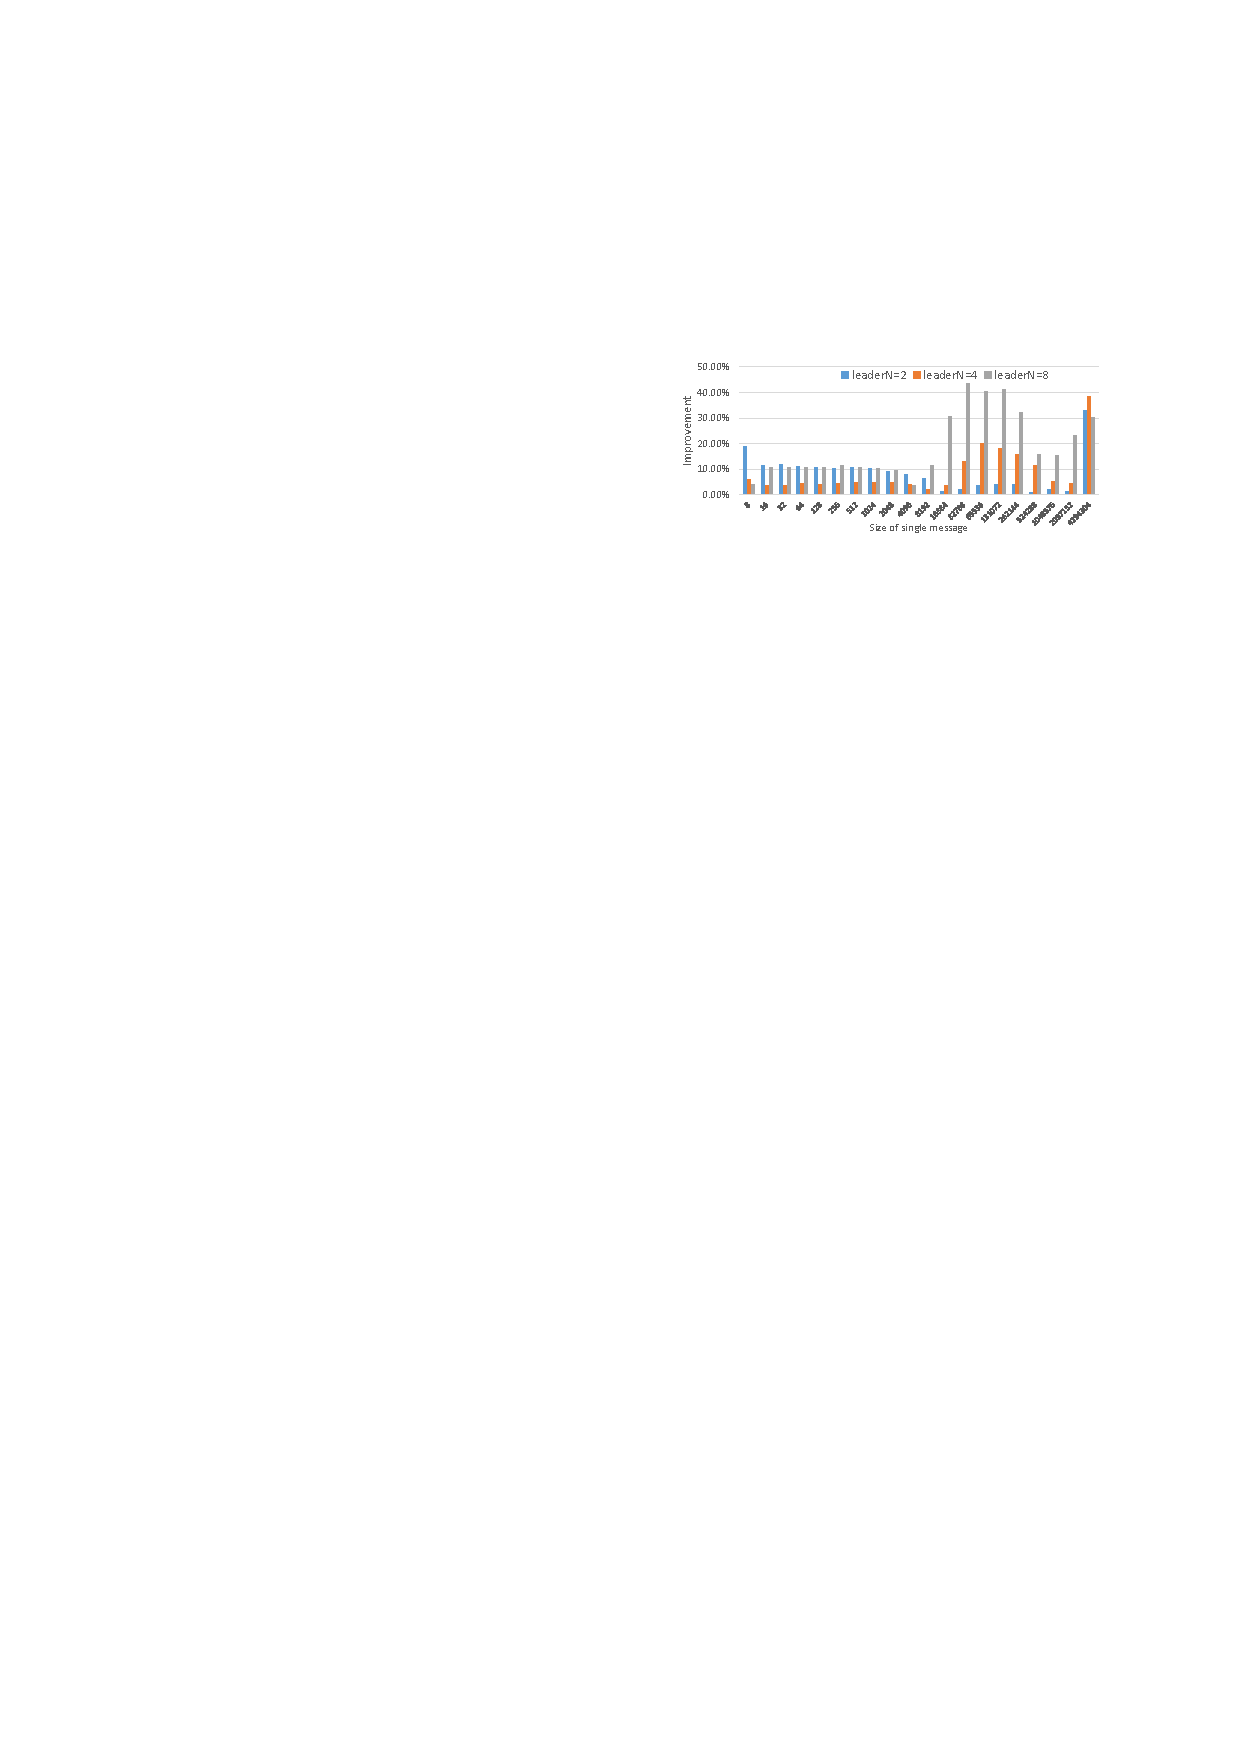
\includegraphics[width=0.49\textwidth]{./Figures/hpcd/NUMA-aware-gather-scatter.pdf}}
  \caption{NUMA-aware multi-leader gahtering/scattering throughput compared to multi-leader gahtering/scattering.}
	\label{NUMA-aware-multi-leader}
	\vspace{0.2in}
\end{figure*}

Morden interconnect network on supercomputer usually have multiple endpoints for each nodes.
Multiple endpoints improve the concurrent ability to process multiple communication requests.
We uses two nodes, one nodes activate several processes to concurrently send to corresponding processes on another node.
As each process in a nodes will activate a network endpoints, the number of activated processes number in a node is equal to the number of network endpoint in using.
As Figure \ref{Multi-port} show, we find that multiple endpoints do improve the node-to-node throughput in most cases.
\begin{figure*}[!htb]
  \centering
    \subfigure[HPC-A 4 NUMAs in a node]{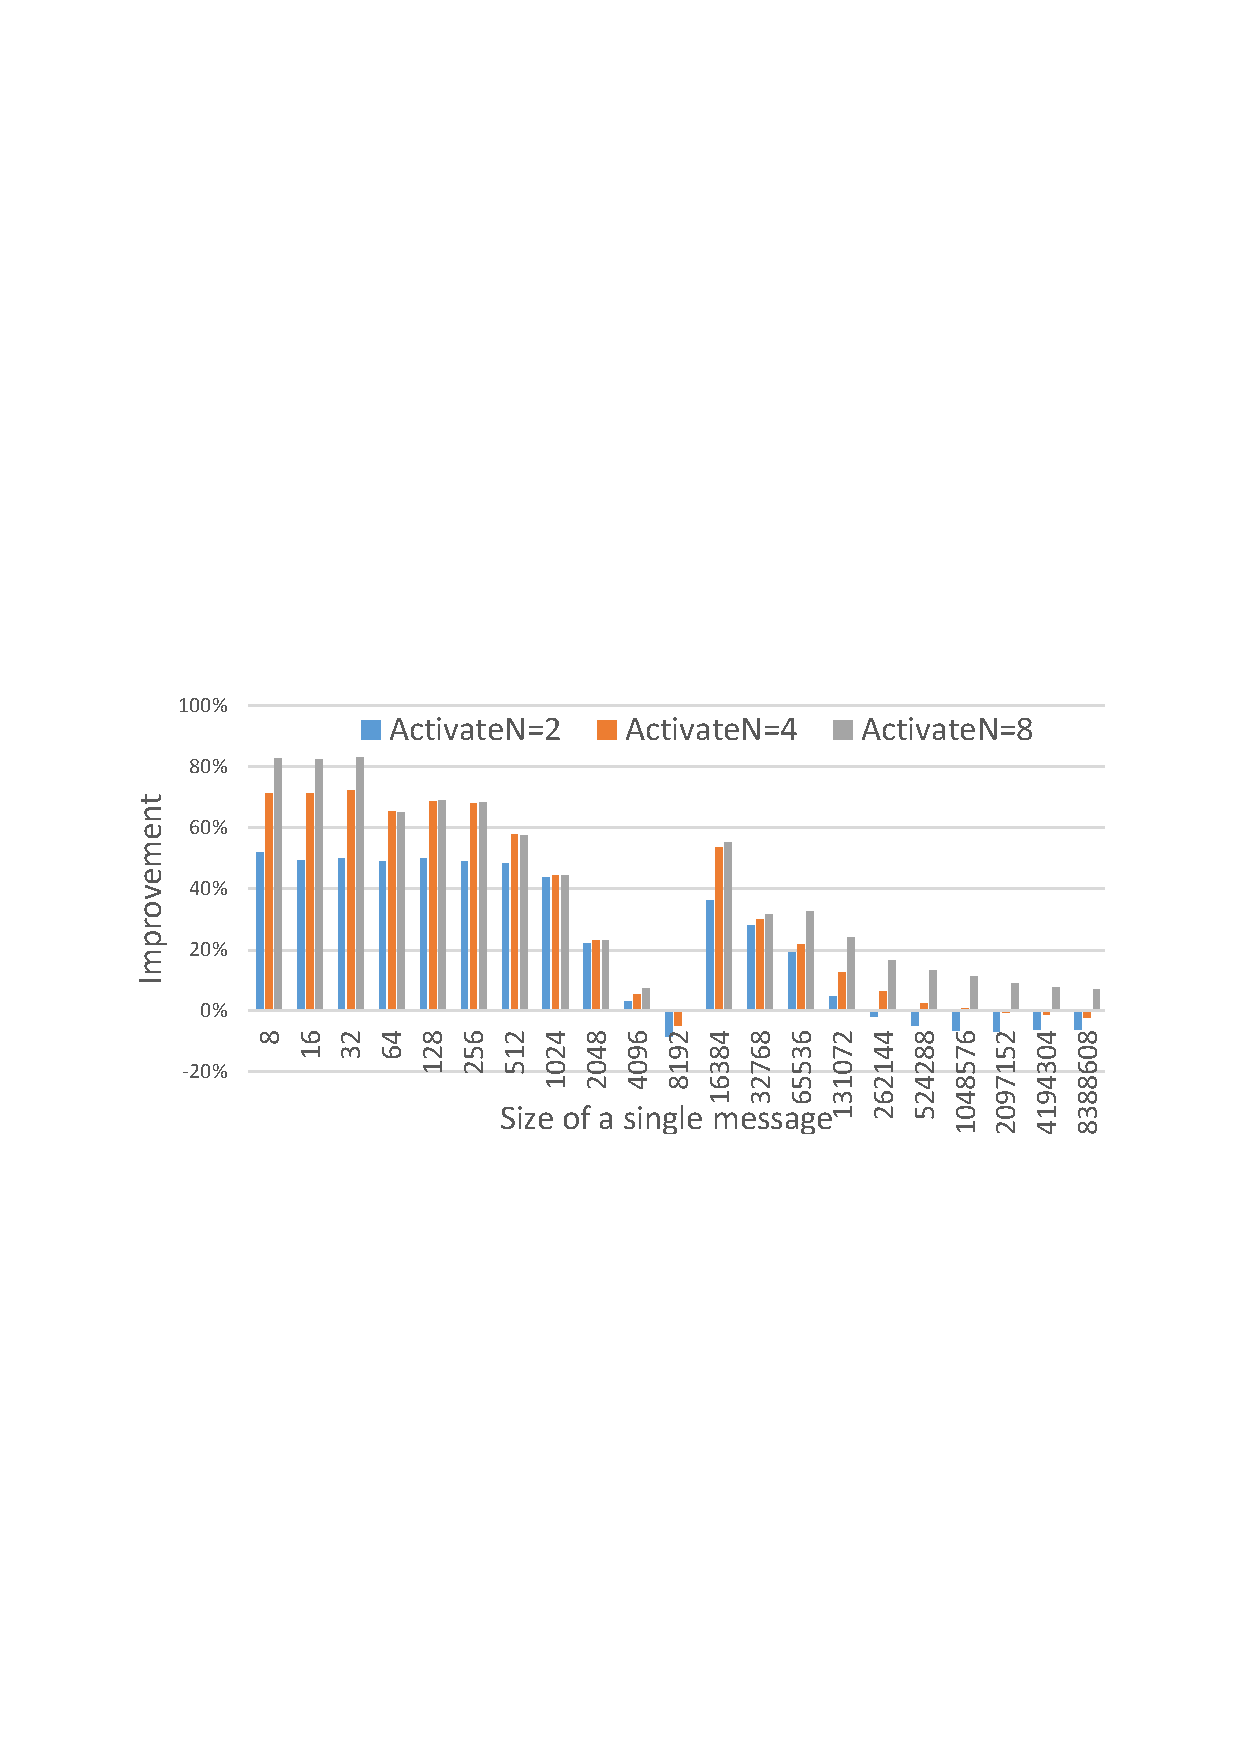
\includegraphics[width=0.49\textwidth]{./Figures/hpca/Multi-port-p2p.pdf}}
	\subfigure[HPC-B 2 NUMAs in a node]{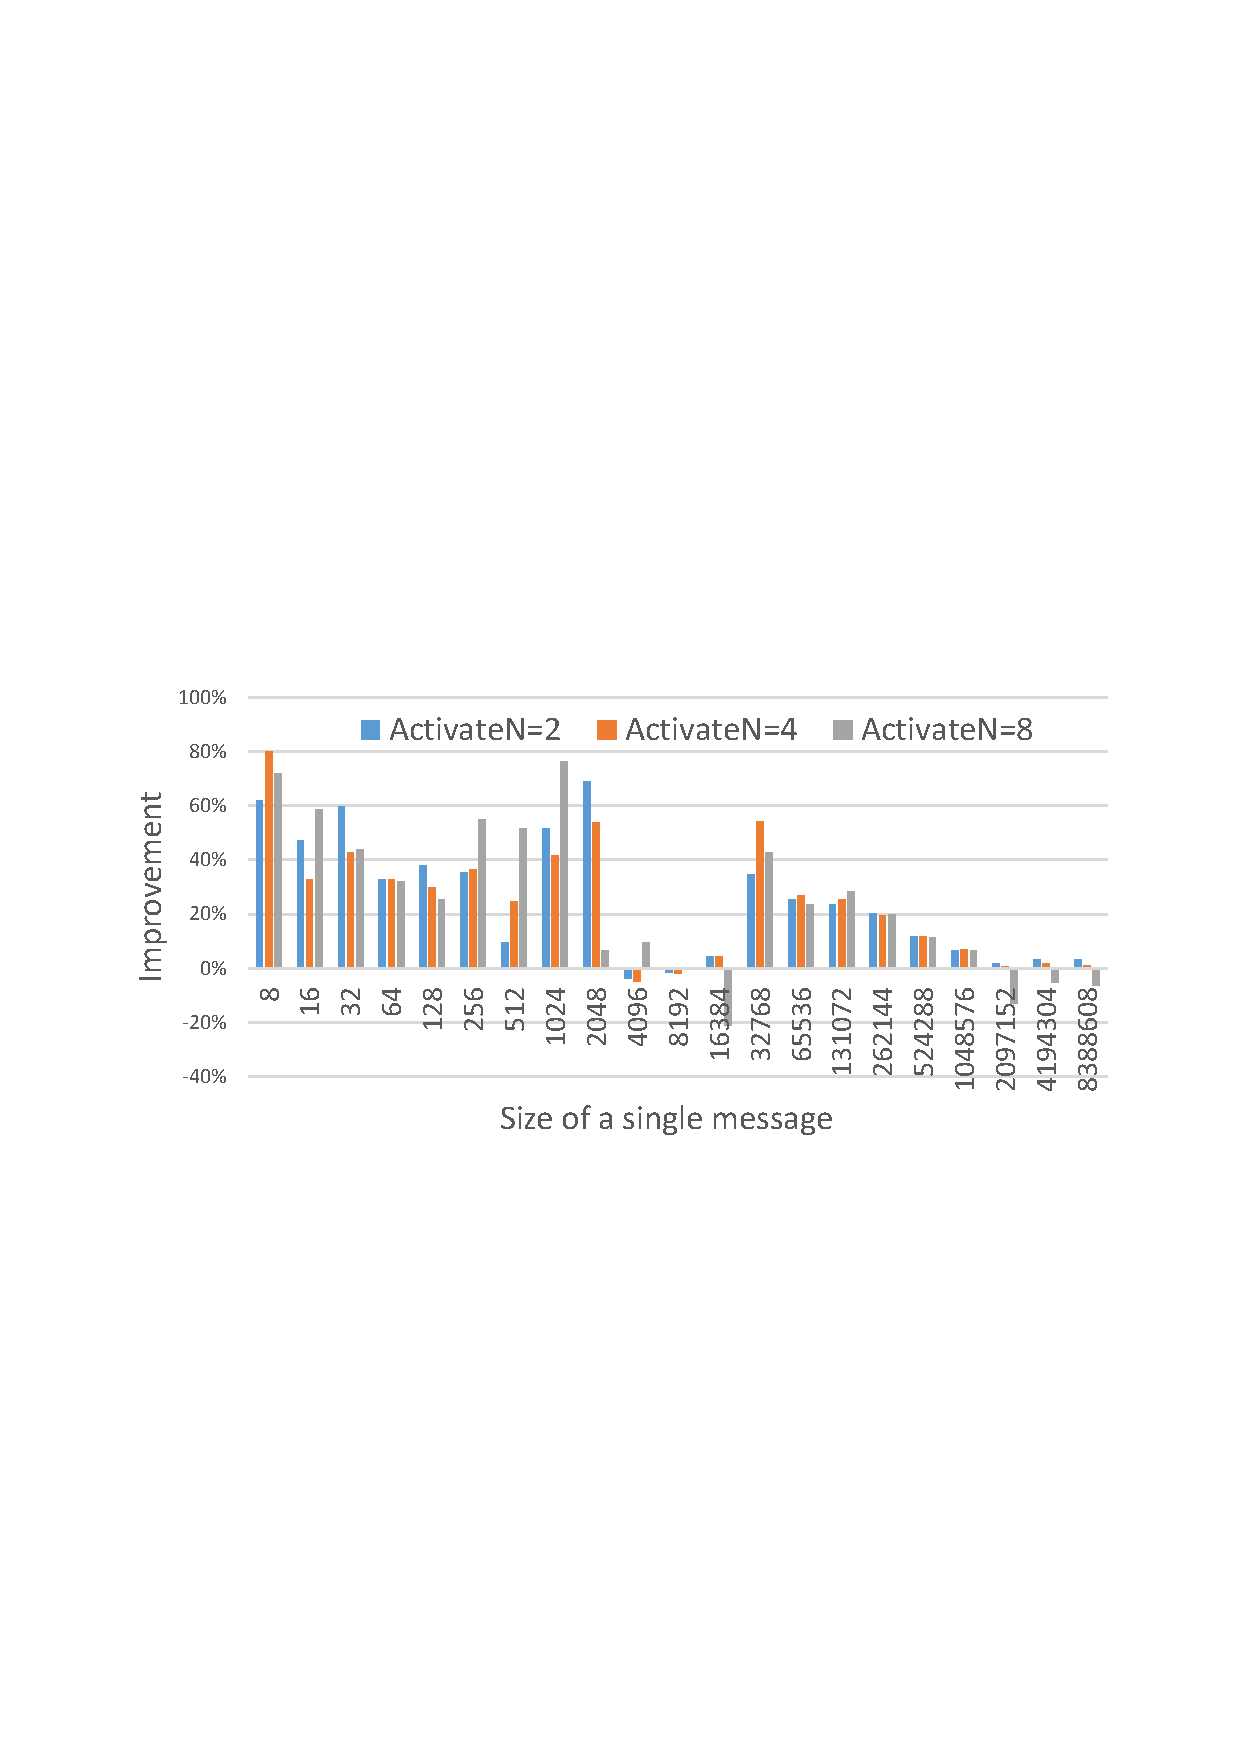
\includegraphics[width=0.49\textwidth]{./Figures/hpcd/Multi-port-p2p.pdf}}
  \caption{Multiple endpoints delivery throughput compared to single endpoints.}
	\label{Multi-port}
	\vspace{0.2in}
\end{figure*}

Besides, as the intra-node communication can be overlappable with inter-node communication, gathering/scattering overhead can be overlapped with inter-node overhead.

Although there are a lot of parallelism, there is no method using all these parallelism to optimize the communication performance of all-to-all.

\section {Gather-Scatter-based Multi-leader all-to-all algorithm}
\subsection{Leader-based All-to-All Collective (L-a2a)}
In this section, we present the Leader-based all-to-all design.
Its algorithm is shown in Algorithm \ref{algorithm-node-aware}.



In algorithm \ref{algorithm-Leader-based}, the first step is a gathering procedure.
In each loop i, all message which need to be sent to node i are gathered into leader ranks of each node and transpose blocks sequentially.
The second step is a inter-node all-to-all between node-leaders.
In each loop i of the final step, messages which received from node i are scattered to the corresponding processes. 



\begin{algorithm}
 \caption{Leader-based All-to-All (L-a2a)}\label{algorithm-Leader-based}
\SetAlgoLined
\SetKwProg{Def}{def}{:}{}
\Def{All-to-all(SendBuf,RecvBuf,count,type,comm)}{
	\For{i in range(0,nodeN)}
	{
		Gather(SendBuf,gather\_result,intra\_node)\;
		transpose(gather\_result,BufferS)
	}
	\If{$myrank $==$ leader$}{Alltoall(BufferS,BufferR,inter\_node)}
	\For{i in range(0,nodeN)}
	{
		Scatter(BufferR,RecvBuf,intra\_node)
	}
}
\end{algorithm}
\begin{algorithm}
\caption{Leaders Placement of MPML}\label{Multi-leader-placement}
\SetKwProg{Def}{def}{:}{}
\Def{am-i-leader(intra-rank)}
{
	\If{intra-rank $<$ LeaderN}{
		return True
	}
	return False
}
\Def{my-leader-id(intra-rank)}
{
	return intra-rank
}
\end{algorithm}

The advantage of leader-based all-to-all collective are:
\begin{enumerate}[(1)]
\item Compared to direct all-to-all, leader-based  all-to-all reduce the number of message by $M^2$ time (M is the number of processes in each node). 
\item Similar to Bruck algorithm \cite{bruck1997efficient}, leader-based all-to-all aggregate the small message to large message. But leader-based all-to-all has less memory copy. It makes leader-based all-to-all suitable for medium-sized messages.
\end{enumerate}


\subsection{Multi-port Multi-leader All-to-all Collective (MPML)}
For larger messages, L-a2a involve too many intra-node overhead.
As a result, multiple network endpoints and processes can help to push the applicable boundary of gathering/scattering all-to-all futher away.
Multi-leader method is using multiple processes in a node to gather/scatter and transpose data.
Multi-port method is opening up multiple network endpoints by multiple processes which using multiple endpoints to process different communication requests.
MPML algorithm is shown in Algorithm \ref{Multi-leader-placement} and \ref{Multi-leader-based-a2a}  and Figure \ref{fig:MPML}.


\begin{algorithm}
\caption{Multi-port Multi-leader a2a (MPML)}\label{Multi-leader-based-a2a}
\SetAlgoLined
\KwIn{PPN:processes per-node, intra-rank: rank within a node, inter-rank: index of nodex
}
\SetKwProg{Def}{def}{:}{}

\Def {Multi-leader-gather(SendBuf,count)}
{
	MPI\_Win\_fence(intra-node)

	\If{am-i-leader(intra-rank)}
	{
		Lid = my-leader-id(intra-rank)

		\For{i in range(Lid,nodeN,LeaderN)}
		{
			target-node $\leftarrow$ (inter-rank + i) mod nodeN

			k $\leftarrow$ $\frac{i}{LeaderN}$

			shift $\leftarrow$ target-node*count*PPN

			\For {j in range(0,PPN)}
			{
				source $\leftarrow$ (intra-rank + j) mod P

				Get(gatherbuf[k][source],source,shift)
			}
			% 
		}
	}
	MPI\_Win\_fence(intra-node)
		
	Leaders transpose all blocks to BufferS
}
\Def {Multi-port-a2a(BufferS,BufferR)}
{
	\If{am-i-leader(intra-rank)}
	{
		Lid = my-leader-id(intra-rank)

		\For{i in range(Lid,nodeN,LeaderN)}
		{
			k $\leftarrow$ $\frac{i}{LeaderN}$

			target $\leftarrow$  (inter-rank + i) mod nodeN

			source $\leftarrow$  (inter-rank + nodeN - i) mod nodeN

			MPI\_Isend(BufferS[k],target)

			MPI\_Recv(BufferR[k],source)
		}

	}
	
}
\Def {Multi-leader-scatter(Recvbuf,count)}
{
	MPI\_Win\_fence(intra-node)

	\If{am-i-leader(intra-rank)}
	{
		Lid = my-leader-id(intra-rank)

		\For{i in range(Lid,nodeN,LeaderN)}
		{
			source-node $\leftarrow$ (inter-rank + nodeN - i) mod nodeN

			k $\leftarrow$ $\frac{i}{LeaderN}$

			shift $\leftarrow$ source-node*count*PPN

			\For {j in range(0,PPN)}
			{
				target $\leftarrow$ (intra-rank + j) mod P

				Put(BufferR[k][target],target,shift)
			}

		}
	}

	MPI\_Win\_fence(intra-node)
}
\Def{all-to-all(SendBuf,RecvBuf,count,type,comm)}{
	Multi-leader-gather(SendBuf,count,gatherbuf)

	Multi-port-a2a(BufferS,BufferR)

	Local-Transpose(BufferR)
	
	Multi-leader-scatter(Recvbuf,count)
}
\end{algorithm}

\begin{figure}
\centering
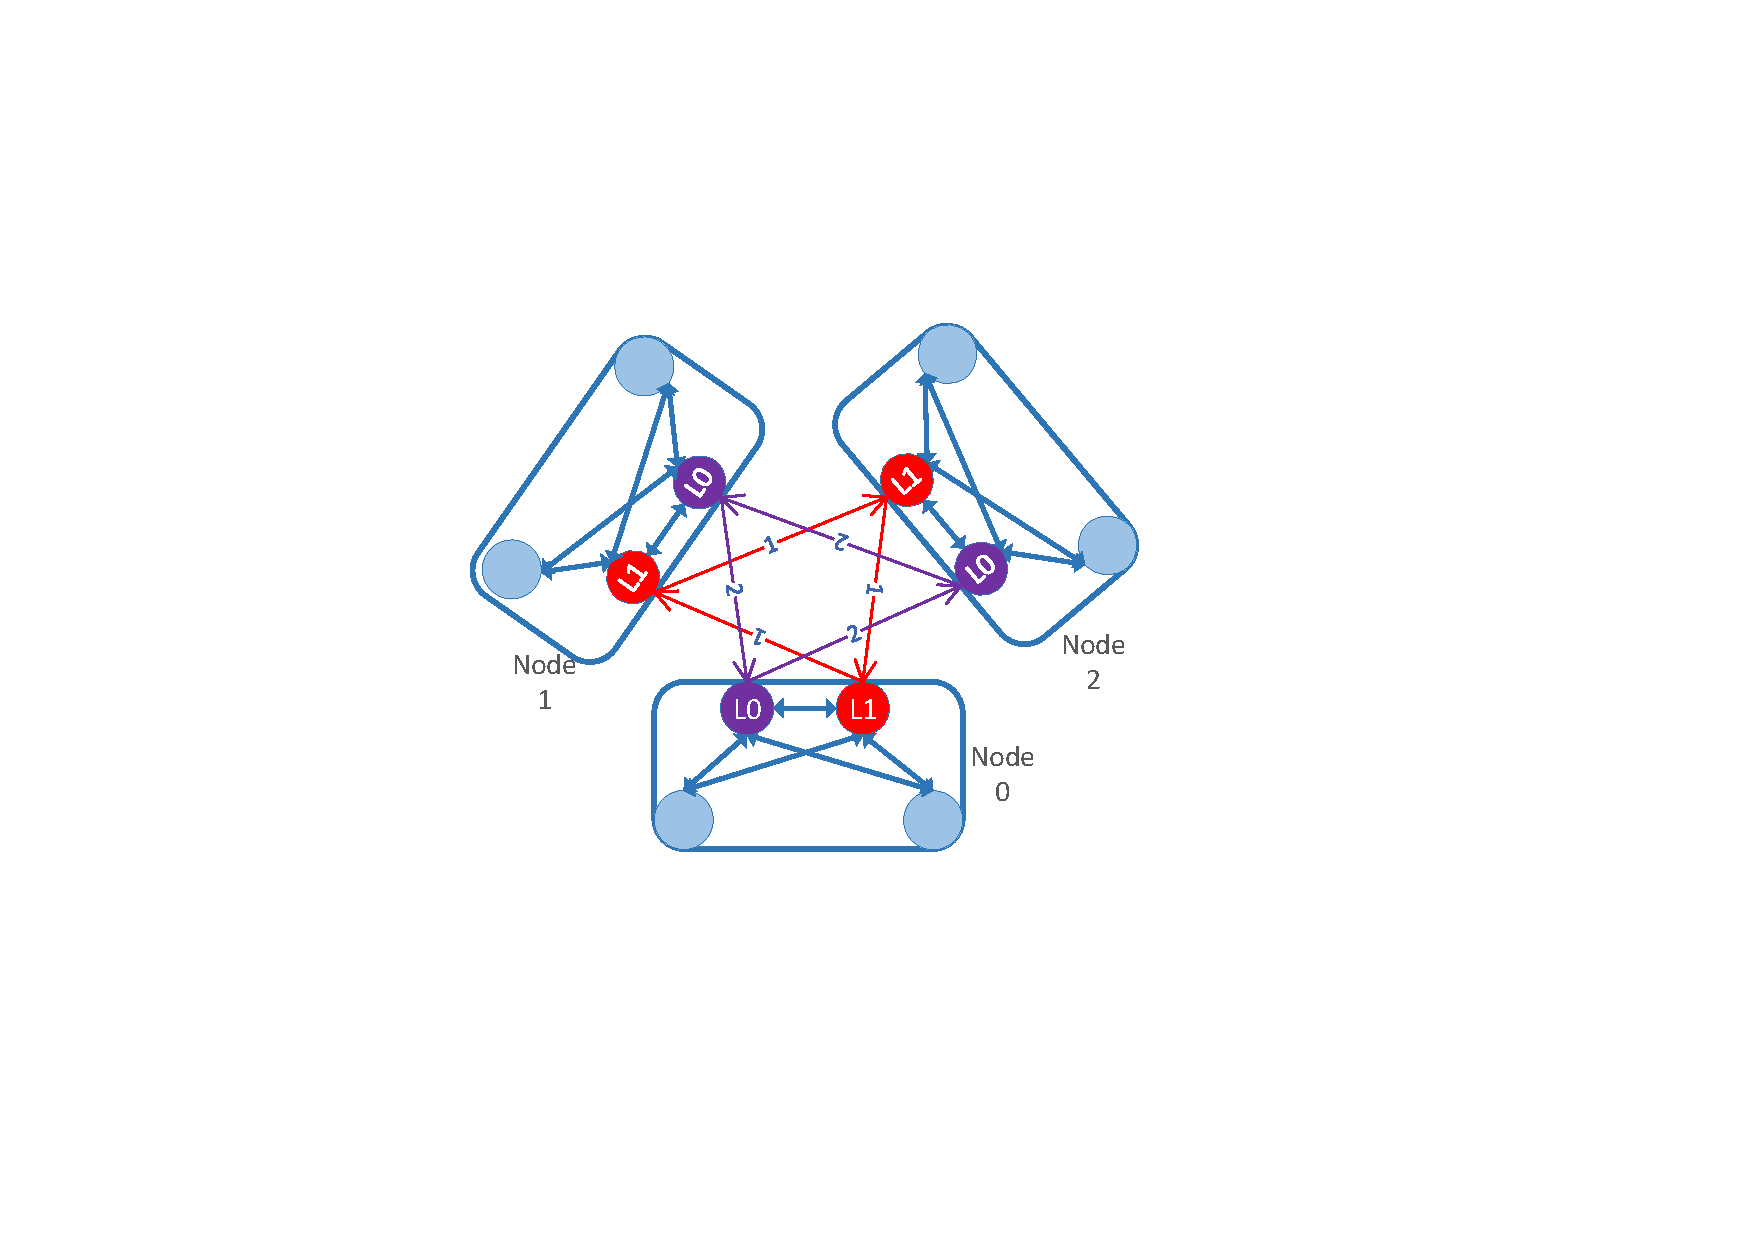
\includegraphics[width=8cm]{./Figures/multi-leader-multi-port-a2a.pdf} %[图片大小]{图片路径}
\caption{Example of 3 nodes 12 processes 2-leader MPML} %图片标题
\label{fig:MPML}
\end{figure}
As shown in Figure \ref{fig:MPML}, there are 2 leaders in a node, different processes are responsible for communicating with different nodes in a round-robin way.
Assume node A send a aggregated message to Node B where B equal to (A + i) mod NodeN.
Leaders i in node A and B are responsible for send and recv the message.


Compared to L-a2a, MPML takes advantage of multi-leader and multi-port to optimize L-a2a.
As disscussed in Motivation part, using multiple processes can improving the gathering and scattering throughput a lot in all message size and HPC we tested. 
Besides, using multiple processes to transpose the local blocks can parallise the local stransposing processes.
Multiple network endpoints can parallelize the startup overhead of multiple communication requests.


% \begin{figure}
% \centering
% % \subfigure[Example of 3 nodes 4 processes L-a2a]{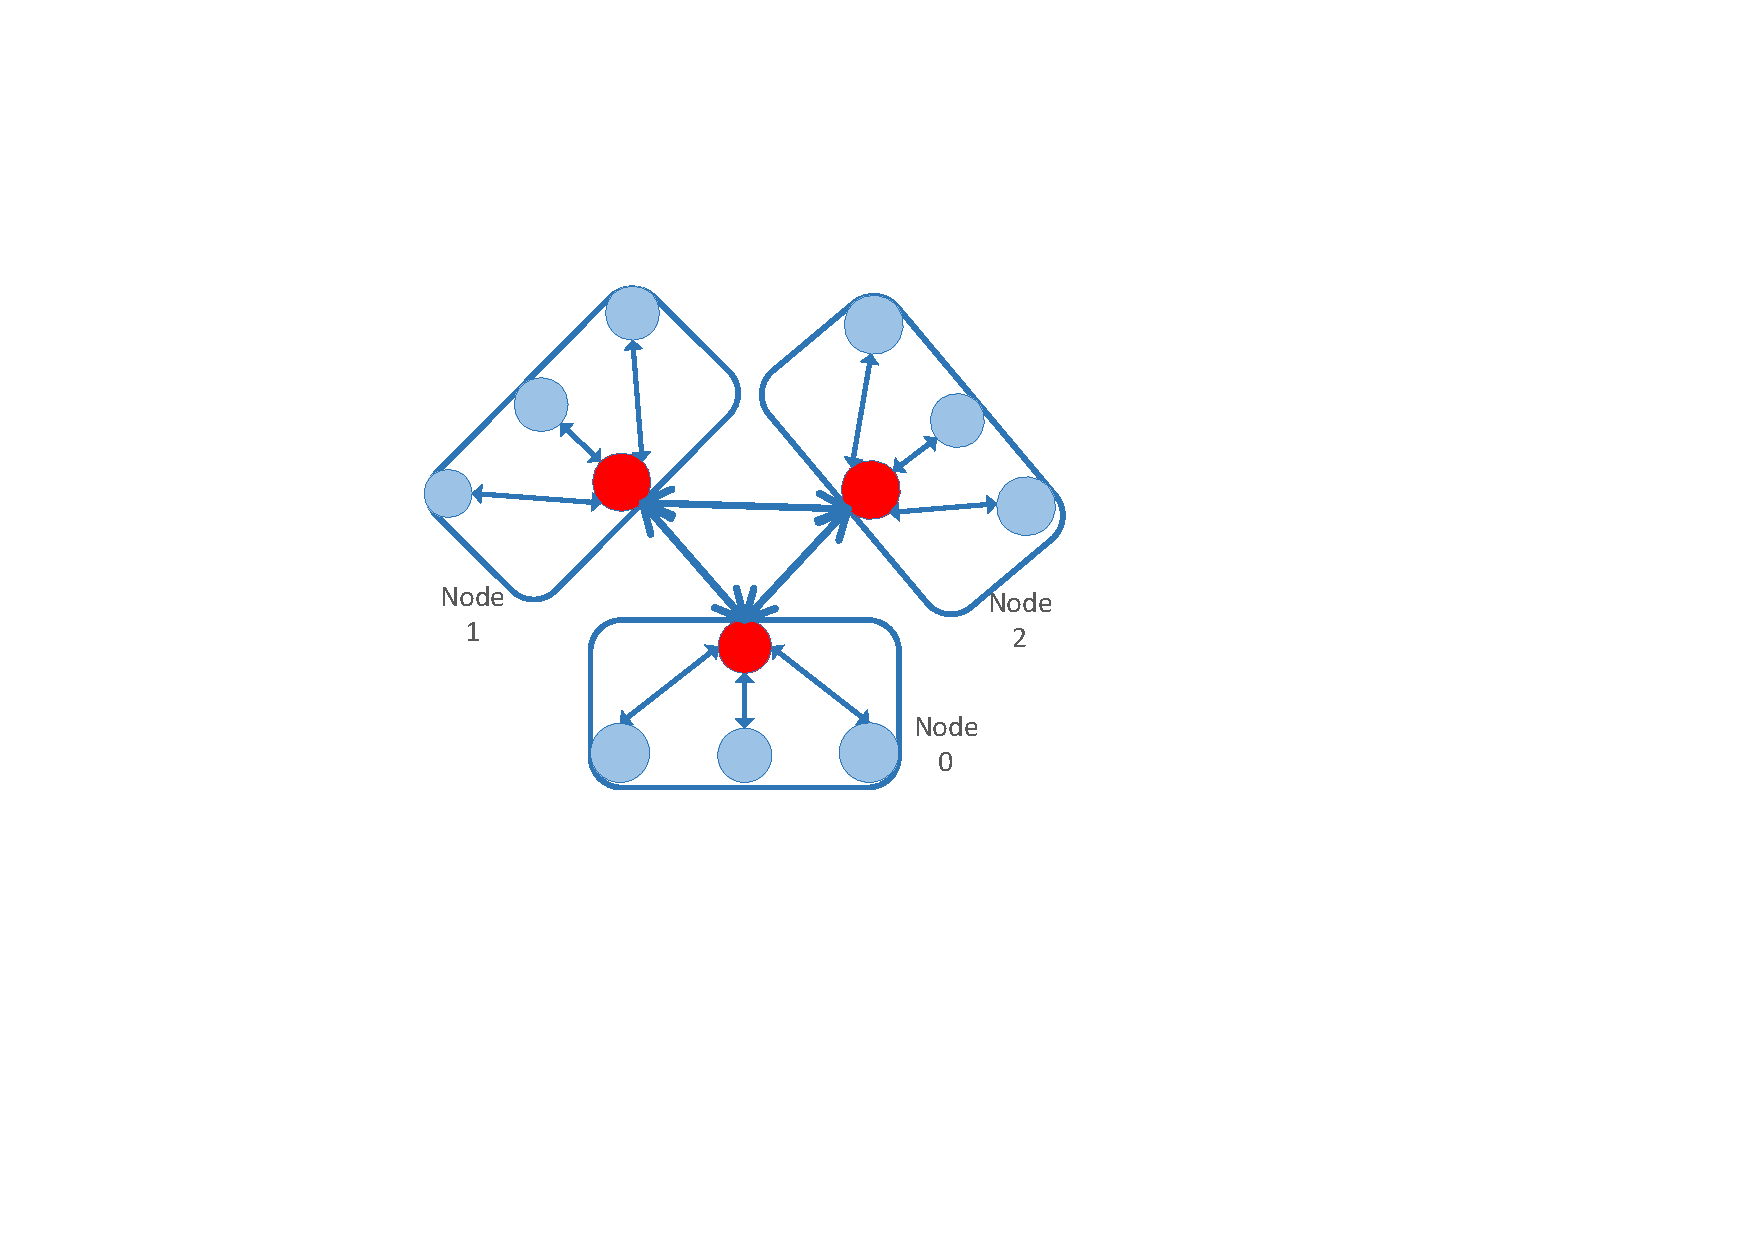
\includegraphics[width=4cm]{./Figures/leader-based-a2a.pdf}}
% \subfigure[Example of 3 nodes 4 processes MPML]{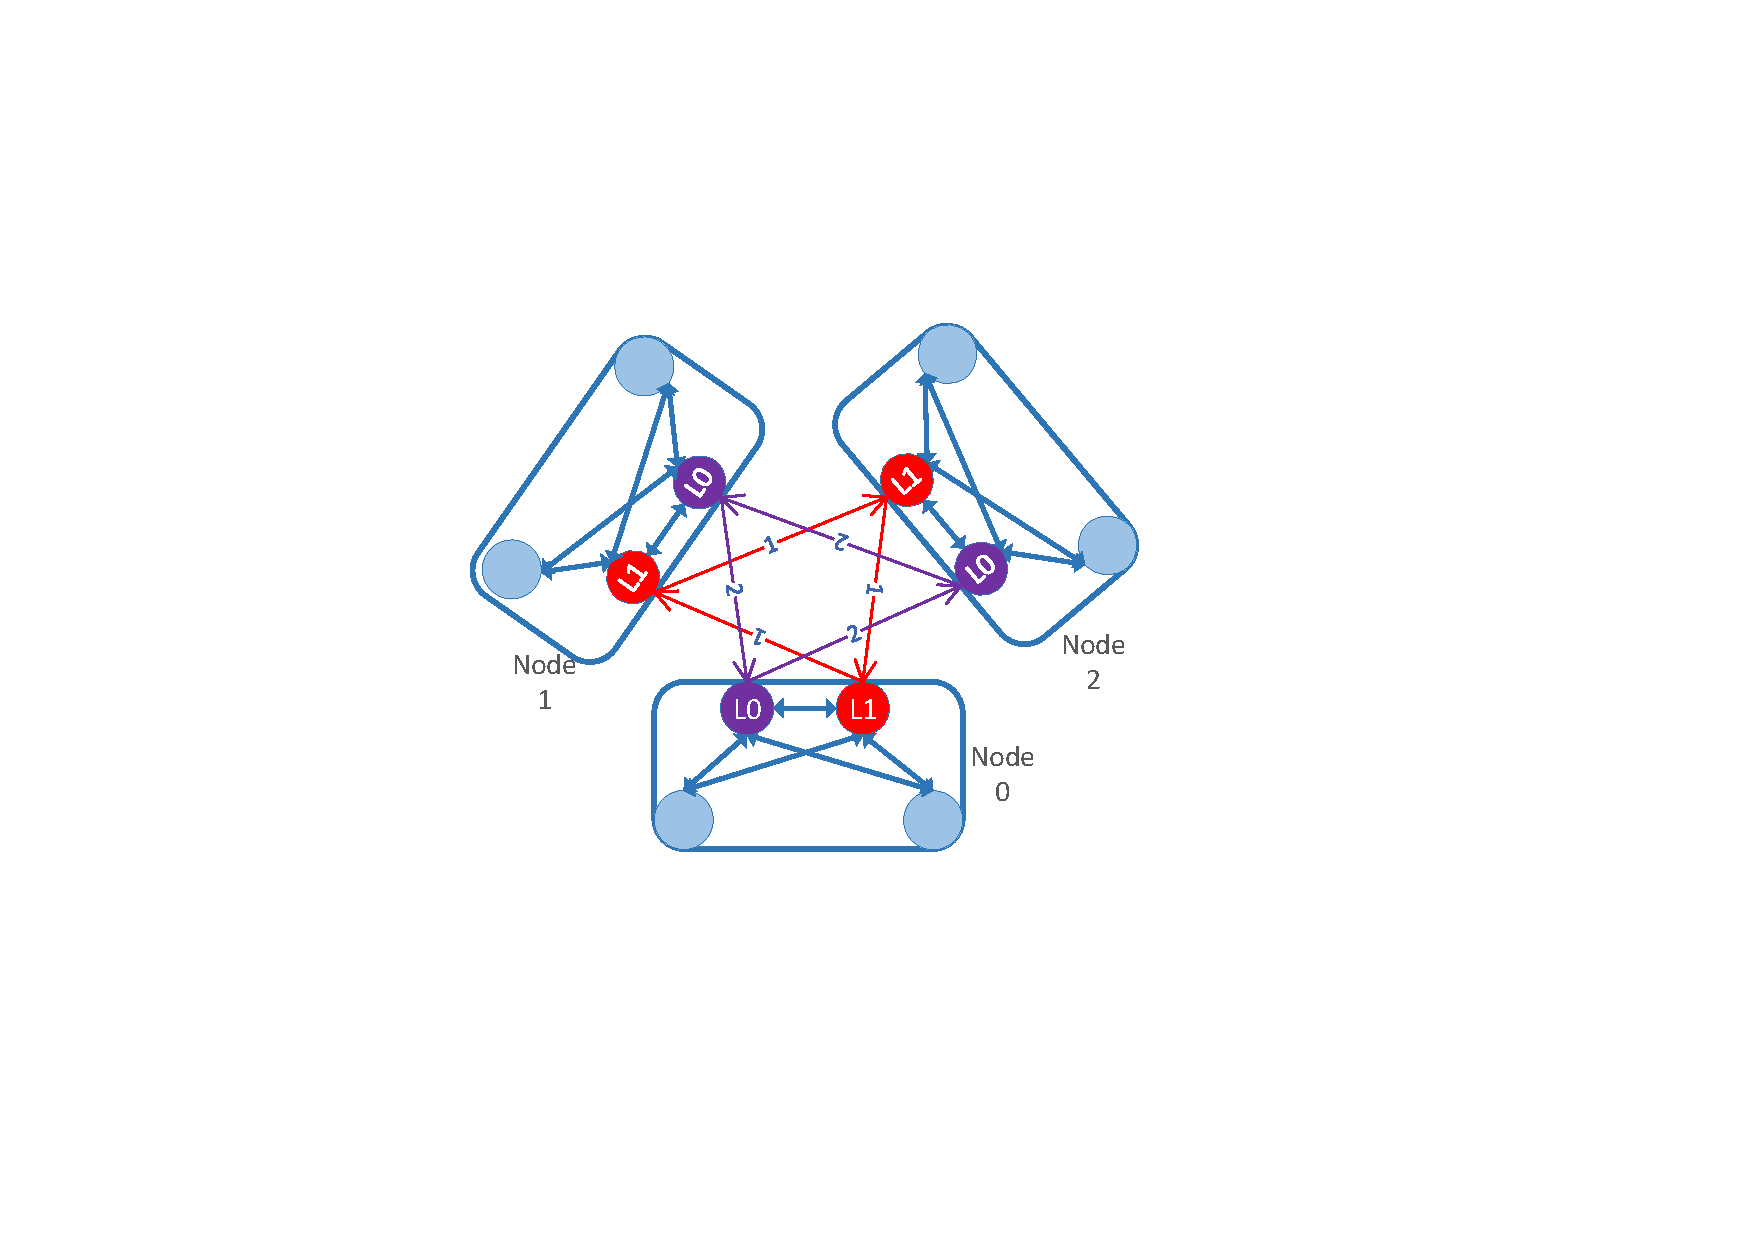
\includegraphics[width=8cm]{./Figures/multi-leader-multi-port-a2a.pdf}}
% % \caption{Jackson Yee} %图片标题
% \label{fig:1}  %图片交叉引用时的标签
% \end{figure}

\subsection {NUMA-aware MPML all-to-all collective (NMPML)}
There are usually NUMA architecture on mordern multi-core processes on supercomputers.
As different CPU has different count of NUMA.
We uniformly spread the leaders on a node to make them utilize all NUMAs.
The core idea can be shown as Figure \ref{fig:NUMA-Aware}.
\begin{figure}
\centering
\subfigure[4 leaders on a 4 NUMA 16 core processor]{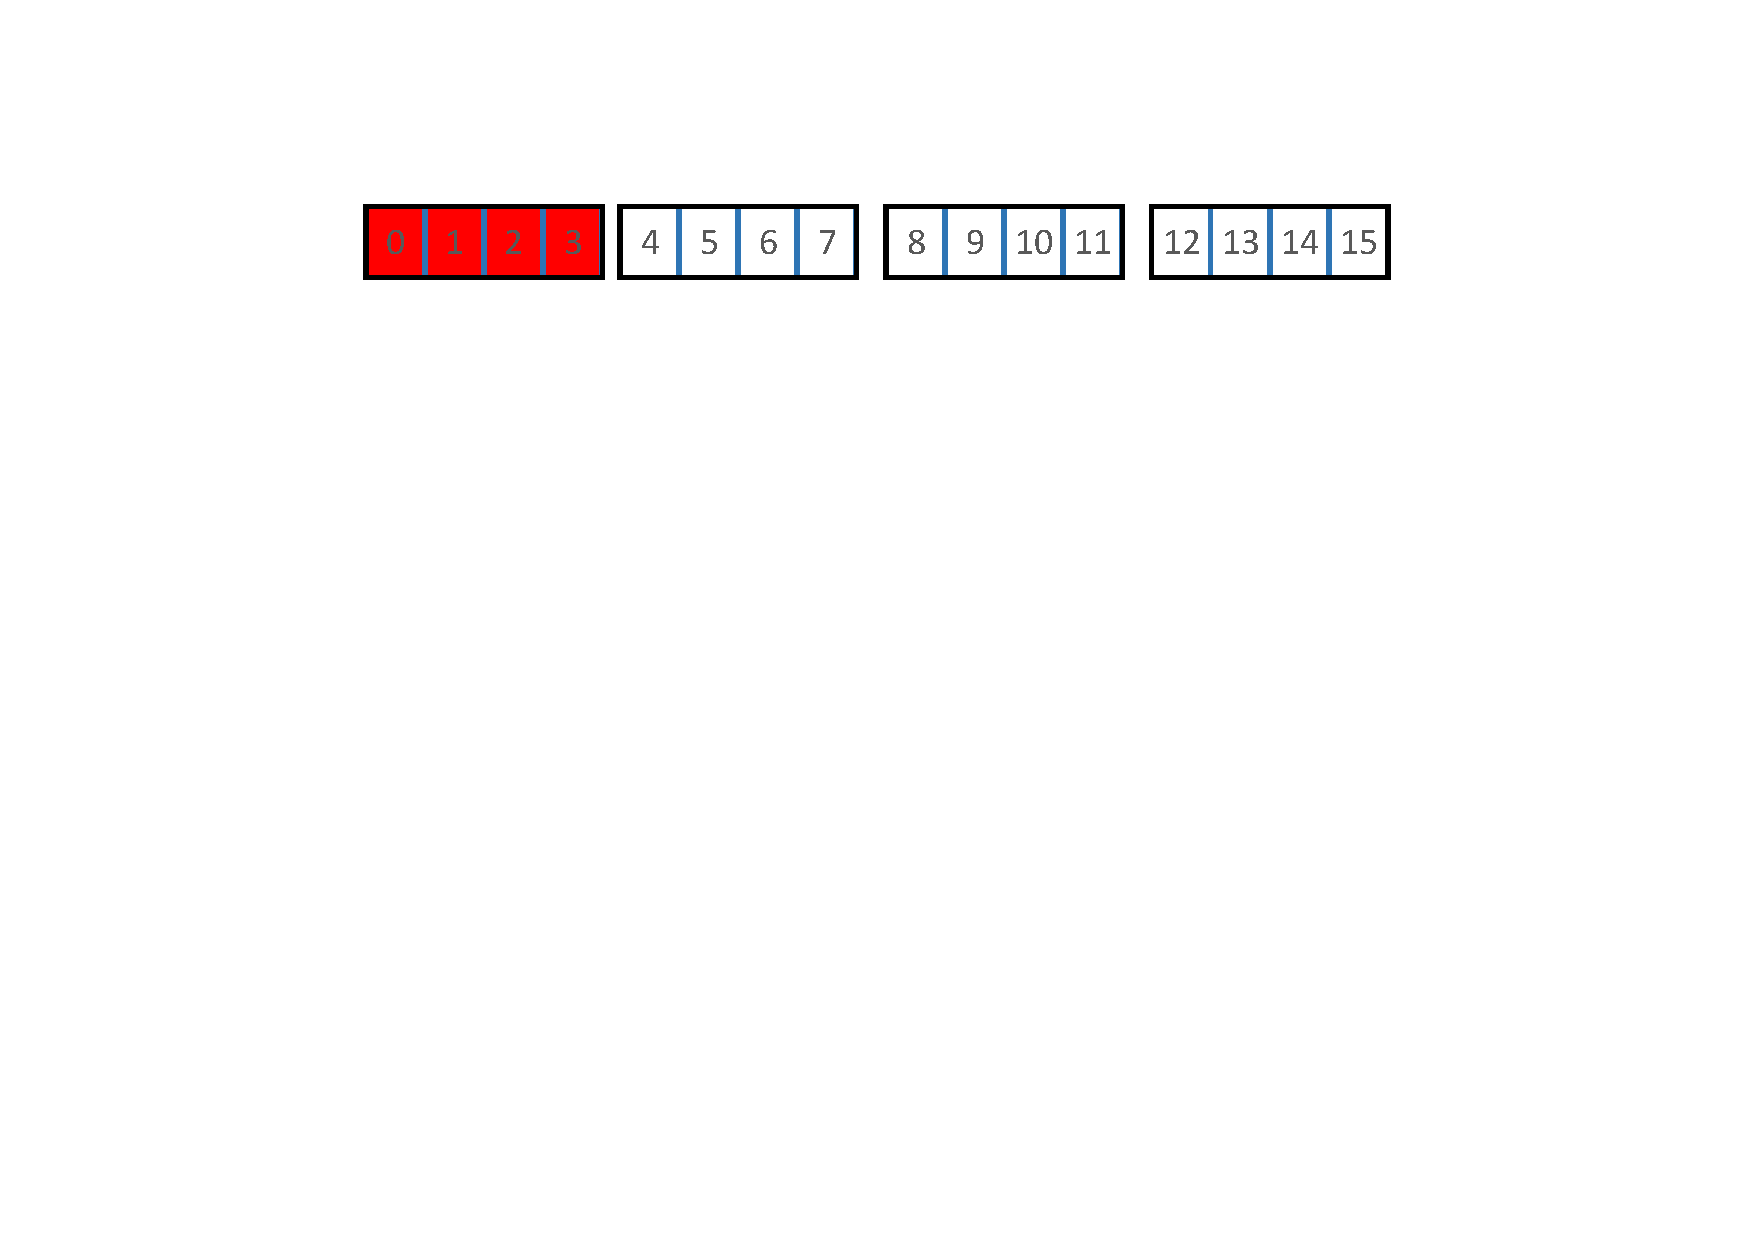
\includegraphics[width=8cm]{./Figures/no-NUMA-awarea2ax.pdf}}
\\
\centering
\subfigure[spreaded 4 leaders on a 4 NUMA 16 core processor]{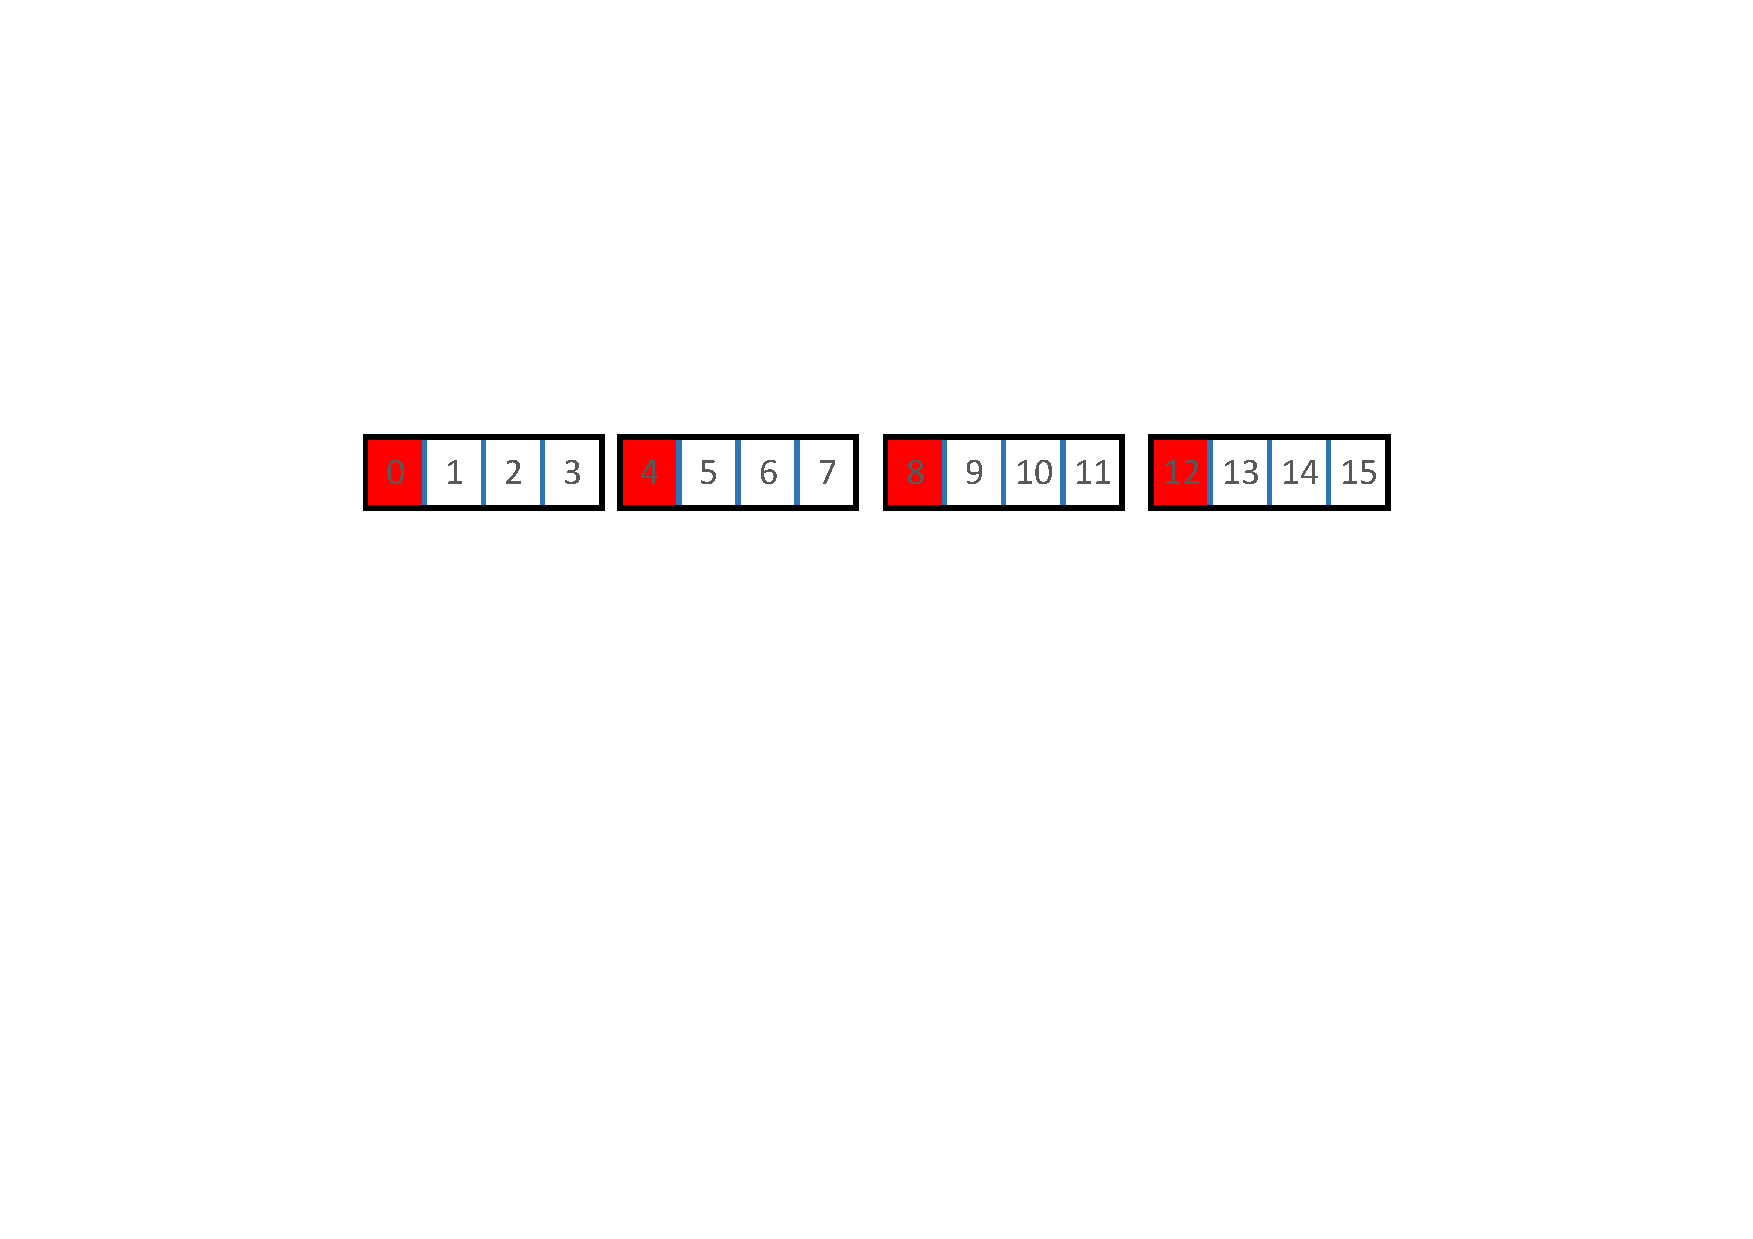
\includegraphics[width=8cm]{./Figures/NUMA-awarea2a.pdf}}
% \caption{Jackson Yee} %图片标题
\caption{NUMA-aware leader placement.} %图片标题
\label{fig:NUMA-Aware}  %图片交叉引用时的标签
\end{figure}

From algorithm view, the only difference between NMPML and MPML is the am-i-leader and my-leader-id functions.
In NMPML, we only to replace the Algorithm \ref{Multi-leader-placement} into Algorithm \ref{NMPML-Multi-leader-placement}.
\begin{algorithm}
\caption{Leaders Placement of NMPML}\label{NMPML-Multi-leader-placement}
\SetKwProg{Def}{def}{:}{}
\Def{am-i-leader(intra-rank)}
{
	dist $\leftarrow$  max($\lfloor \frac{intra-procn}{leaderN} \rfloor$, 1) \\
	t $\leftarrow \frac{intra-rank}{dist}$ \\
	r $\leftarrow$ intra-rank mod dist \\
	\If{r == 0 and t $<$ leaderN}{ 
		return True
	}
	return False
}
\Def{my-leader-id(intra-rank)}
{
	dist $\leftarrow$  max($\lfloor \frac{intra-procn}{leaderN} \rfloor$, 1) \\
	return $\frac{intra-rank}{dist}$
}
\end{algorithm}

As we have discussed in Motivation section, when spreading leaders on the node, we acquire beter gathring/scattering throughput in most cases.

\subsection{Overlapping Intra-node and Inter-node Communication of NMPML (ONMPML)}


We notice that the overead of gathering, scattering, and transpose can be overlapped with inter-node communication.
As shown in Figure \ref{fig:ONMPML}, there are 2 leaders in a node. 
Each leaders send a block immediately after the block is gathered.
\begin{figure*}
\centering
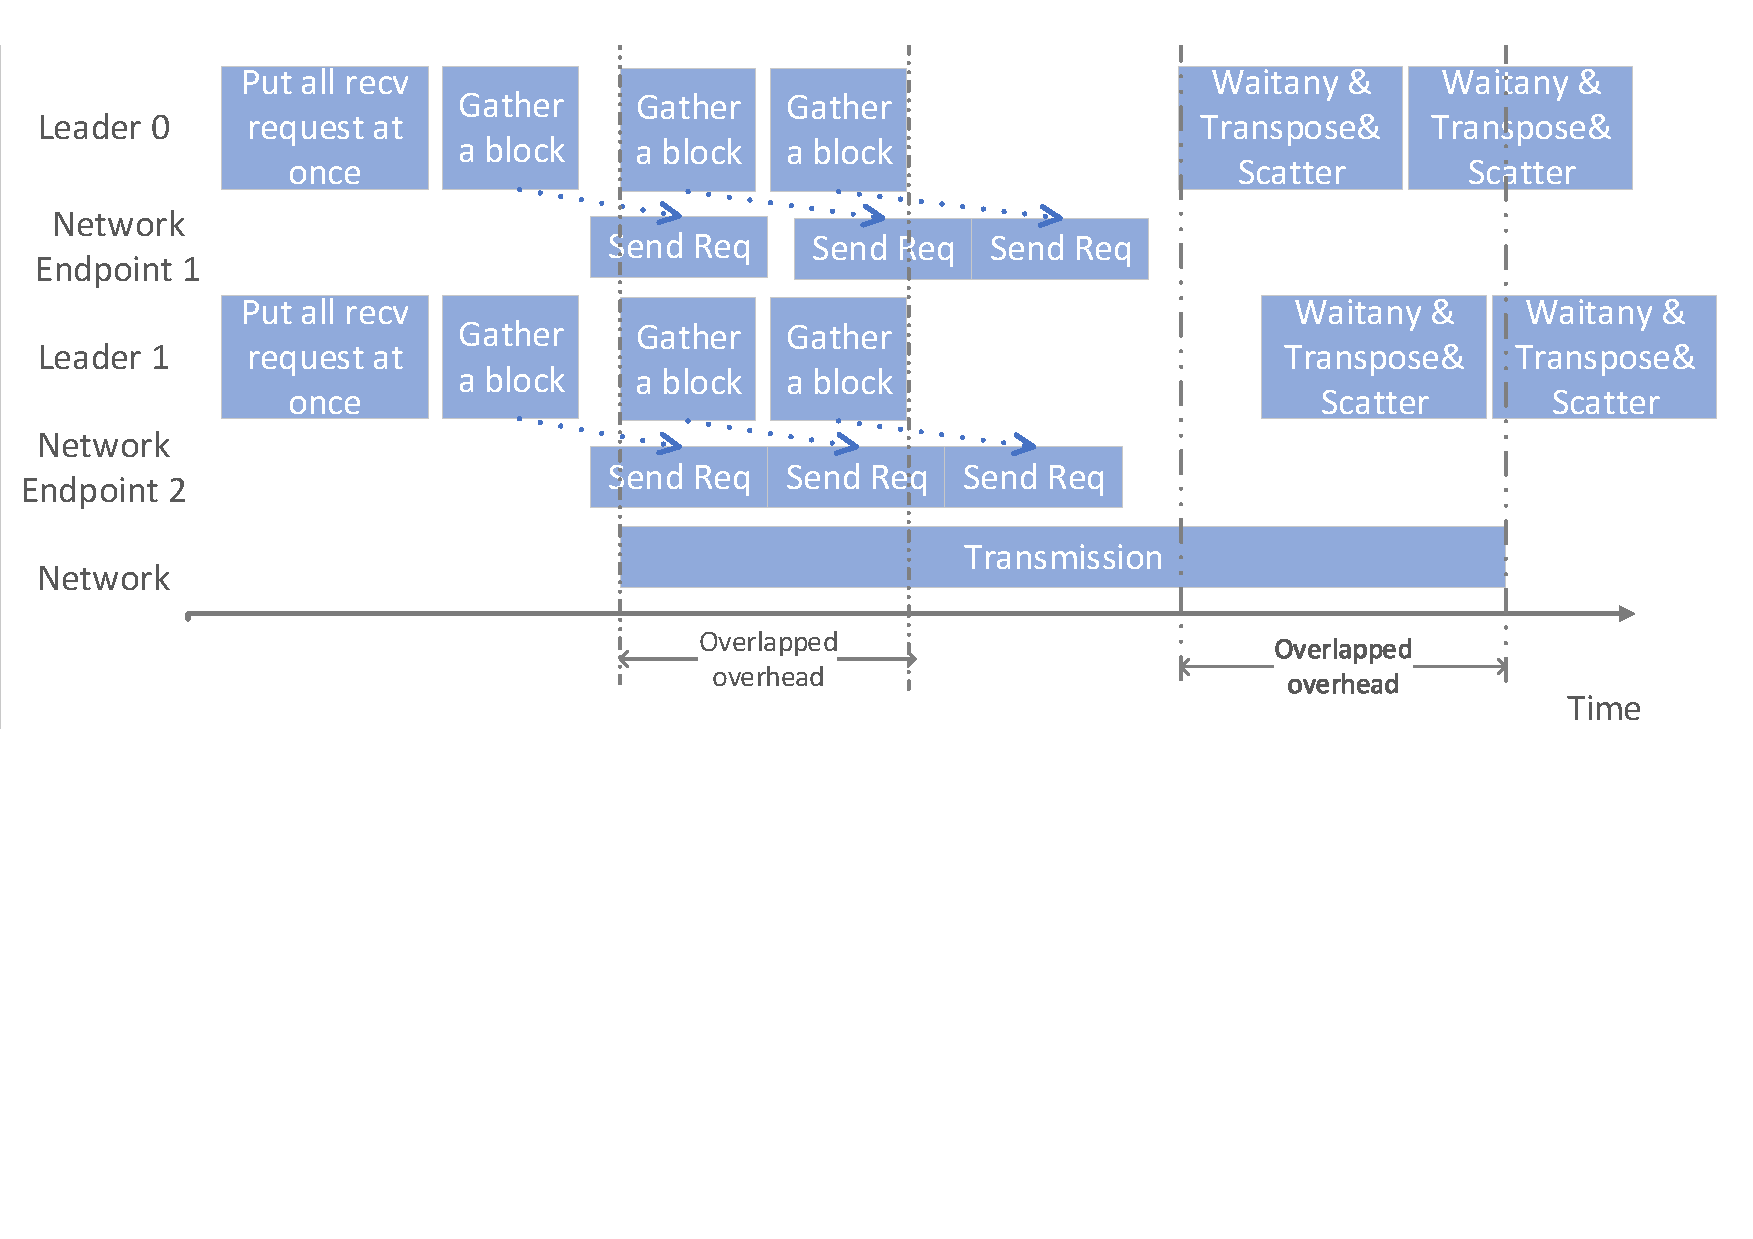
\includegraphics[width=16cm]{./Figures/Overlap-inter-intra-node-communication.pdf} %[图片大小]{图片路径}
\caption{Overlap the intra-node communication and inter-node communication with 2 leaders} %图片标题
\label{fig:ONMPML}
\end{figure*}

In Figure \ref{fig:ONMPML}, assume there are 2 leaders and 2 endpoints in a node. 
First, each leaders post all non-blocking receive requests at once.
Then, each leader start gathering data, once a block is aggregated, it sends out the block immediately.
After the first gathering, the second gathering is overlapped with network communication.
As a result, as long as the number of node is big enough, the gathering overhead can be mostly overlapped with inter-node communiation.
As to the scattering overhead, receive leaders start scattering as long as it receive one block.
While in NMPML, receive leaders start scattering data after all blocks arrived.
The throughput of ONMPML depends on  the slowest one: network bandwidth or gather-scattering throughput.

The Algorithm \ref{OverlapedMulti-leader-based-a2a} show the ONMPML algorithm on RMA (intra-node communication) and RDMA (inter-node communication).
Compared to NMPML, ONMPML using nonblock communication (MPI\_Isend/Irecv or RDMA etc.) to overlap the network communication with gathering and scattering procedure.
For gathering and scattering procedure, only leader processes are activated other processes do not participate gathering or scattering.
Remote Memory Access (RMA) makes the leaders can access other processes space directly.

\begin{algorithm}
	\caption{Overlapped NUMA-aware Multi-port Multi-leader a2a (ONMPML)}\label{OverlapedMulti-leader-based-a2a}
	\SetAlgoLined
	\KwIn{PPN:processes per-node, intra-rank: rank within a node, inter-rank: index of nodex
	}
	\SetKwProg{Def}{def}{:}{}

	\Def{all-to-all(SendBuf,RecvBuf,count,type,comm)}
	{
		intra-node-barrier()
		
		\If{am-i-leader(intra-rank)}
		{
			Lid = my-leader-id(intra-rank)

			\For{i in range(Lid,nodeN,LeaderN)}
			{
				target-node $\leftarrow$ (inter-rank + i) mod nodeN

				k $\leftarrow$ $\frac{i}{LeaderN}$

				shift $\leftarrow$ target-node*count*PPN

				\For {j in range(0,PPN)}
				{
					source $\leftarrow$ (intra-rank + j) mod P

					Get(gatherbuf[k][source],source,shift)
				}

				RDMA\_req.target $\leftarrow$ target

				RDMA\_req.event $\leftarrow$ [inter\_rank, k]

				RDMA\_Put(gatherbuf[k],RDMA\_req)
				% 
			}
			\For{i in range(Lid,nodeN,LeaderN)}
			{
				WaitAnyEvent(\&event)

				source-node $\leftarrow$ event[0]

				k $\leftarrow$ event[1]

				LocalTranspose(BufferR[k])


				shift $\leftarrow$ source-node*count*PPN

				\For {j in range(0,PPN)}
				{
					target $\leftarrow$ (intra-rank + j) mod P

					Put(BufferR[k][target],target,shift)
				}


			}
		}
		
		intra-node-barrier()
	}
\end{algorithm}


% Tianhe's RDMA operation provide a capability to control the on going messages number at the same time.
% If we set the ongoing message number to 2, each node can process a communication request as long as there is 0 or 1 requests on going.
% Lesser ongoing message number, the scattering overhead can be better overlapped with communication.
% Because messages arrives more sequentially.
\section{Modeling the performance of all-to-all algorithms on multi-core supercomputer}

In this section, we analyze the performance of traditional algorithms and our algorithms.
We need a model which considering the effect of multiple core, NUMA, and network endpoints.
For inter-node communication, we just using the classical logP model \cite{culler1993logp}.
Classical intra-node communication model cannot meet our needs to model and anylyze our algorithms.
We use the $\tau$-Lop \cite{rico2015tau} to model the intra-node communication.

\subsection {The parameters of the model}
In $\tau$-Lop \cite{rico2015tau}, there are several definition we need to use:
\begin{enumerate}[(1)]
\item $L(m,\tau)$ is cost to concurrently transfer $\tau$ messages with size m. There is a equation in $\tau$-Lop: 
\begin{equation}
\label{concurrently-p2p}
\begin{split}
L(m,1) \le L(m,A) \le A\times L(m,1)
\end{split}
\end{equation}
It means that sending a message with size m is faster than concurrent sending $A$ messages with size m. 
Concurrent sending $A$ messages with size m is faster than seperate sending A messages with size m.
\item n is the number of data transfers time neededs to move from send buffer to the receive buffer. 
For kernel-assistant or shared-heap-based intra-node communication, n equals to 1.
Because a process can directly access other processes memory space, a process only need one copy to sending or receiving a message.
For POSIX shared memory, n equals to 2.
Because data on send buf has to be copied onto a shared buffer, then the receiving process copy the data from shared buffer to receive buffer.
\item k, the number of segments the message is split into.
\item o(m) is the time elapsed since the invoking of a message transmission operation until the beginning of data injection into the channel.
\end{enumerate}
The time to send a intra-node message with size m is:
\begin{equation}
\begin{split}
T(m) = o(m) + \sum_{j=0}^{k+n-2}L_j(\frac{m}{k},\tau{_j})
\end{split}
\label{intra-p2p}
\end{equation}
In POSIX shared memory, where n = 2, equation \ref{intra-p2p} becomes:
\begin{equation}
\begin{split}
T(m) = o(m) + 2L(S,1) + (k-1)L(S,2)
\end{split}
\label{real-p2p}
\end{equation}

When concurrently transer A messages, its overhead defined as $A||T(m)$, which is: 
\begin{equation}
\label{intra-concurentp2p}
\begin{split}
A||T(m)  = o(m) + \sum_{j=0}^{k+n-2}L_{j}(m,A\tau_j)
\end{split}
\end{equation}

Through equation \ref{concurrently-p2p} and \ref{intra-concurentp2p}, we have:
\begin{equation}
\label{concurent-unequation}
\begin{split}
A||T(m)  \le A \times T(m) 
\end{split}
\end{equation}


For inter-node communication, we using logP model.
Some other definition we need are:
\begin{enumerate}[(1)]
\item M, the number of nodes.
\item p, the total number of processes.
\item ppn, the number of processes in each nodes.
\item nn, the number of NUMAs in each nodes. 
\item n1, the number of processes in a NUMA.
\item ln, the number of leaders and network endpoints used in each nodes. We usually have $ln \le nn$.
\item sz, the all-to-all message size between a pair of processes.
\item $b'$, the thoughput of transposing a buffer. $b' * m$ is the overhead to transpose a buffer where its length is m.
\end{enumerate}

Beside, in order to ensure the consistency of the algorithms, assuming all intra-node gatering/scattering operations in L-a2a, MLMP, NMLMP, ONMLMP are based on direct algorithm.
The inter-node alltoall are based on pairwise algorithm.
\subsection {Overhead of direct pairwise all-to-all}

Direct all-to-all takes p step to finish the communication.
In step i, rank j send a message to rank (j+i) mod p and receive a message from rank (j+p-i) mod p.
We consider the MPI rank is uniformly spreaded on the node.
The overhead of first step where each processes send a message to themself is ignored. 
For step 1, there is one outgoing message from a node.
For step ppn, there are ppn  messages outgoing from a node.
When p larger than ppn, there are still ppn messages outgoing from a node.
If we consider the inter-node bandwidth is smaller than intra-node bandwidth, we have:
The overhead of step i ($i < ppn$) is: $i\times L + o + i(sz-1)\times G + g$.
The overhead of step i ($i \ge ppn$) is: $ppn\times L + o + ppn(sz-1)\times G + g$.
As a result, the total overhead of direct all-to-all is:
\begin{equation}
\label{direct-all-to-all}
\begin{split}
T_{d-a2a}(sz)  & = 2*\sum_{i=1}^{ppn-1} (i\times L + o + i(sz-1)\times G + g) \\ 
				 & + \sum_{i=1}^{p + 1 - 2ppn}(ppn\times L + o + ppn(sz-1)\times G  + g)  \\
				 & = ppn \times (p - ppn) \times (L + G \times(sz - 1)) \\
				 & + (p - 1)(o + g)  \\
				 & \approx ppn \times (p - ppn) \times (L + G \times sz) + p\times(o+g)
\end{split}
\end{equation}

\subsection {Overhead of leader-based all-to-all (L-a2a)}

As we are considering direct Gather/Scatter algorithm, in $\tau$-lop, the overhead to gather/scatter one block is: $ppn||T(sz\times ppn)$.
This means that, there are ppn concurent messages, the size of each message is $sz\times ppn$.
As there are M blocks in a node, overhead to gather/scatter M blocks is: $M\times (ppn||T(sz\times ppn))$.
The LogP overhead of inter-node pariwise all-to-all is: $(M-1) \times (L + o +(size - 1) \times G + g) \approx (M-1) \times (L + o +size\times G + g)$.
Overall, the overhead of L-a2a is O(gather) + O(transpose) + O(inter-node alltoall) + O(scatter) which is :
\begin{equation}
\begin{split}
T_{L-a2a}(sz) & = M\times (ppn||T(sz\times ppn)) \\
			  & + M\times b'\times sz\times ppn\times ppn \\
			  & + (M-1) (L + o +(sz\times ppn\times ppn - 1) \times G + g) \\
			  & + M\times (ppn||T(sz\times ppn))  \\
\end{split}
\label{L-a2a-overhead}
\end{equation}

Compared to $T_{d-a2a}$, $T_{L-a2a}$ has same coeffient of G, which is the overhead on the network.
L-a2a has a far less message number than d-a2a.
But L-a2a incurs a lot gathering/scatering overhead.
So, for small message and medium message, L-a2a may have performance improvement than d-a2a.

\subsection {Overhead of  Multi-port Multi-leader a2a (MPML)}

Compared to L-a2a, MPML using multiple process to do gatering, scattering, and transposing operation and using multiple enpoint to concurrently process communication request.
For ppn processes in a node, the first ln processes are chosed to be leader.
For local transpose overhead, the local transpose overhead are evently amortised on multiple pocesses.
For gathering and scattering overhead, as these leaders are placed on a same NUMA, all leaders gathring procedure are concurrently processed.
As for inter-node communication, MPML has lower overhead  of o and g than L-a2a because of using multiple network endpoint.

% When assuming that the number of leader is less than the number of processes in a NUMA.
So the overhead of MPML is:
\begin{equation}
\begin{split}
T_{MPML}(sz) & = 2 \times \frac{M}{ln} \times ((ppn\times ln)||T(sz\times ppn)) \\
			  & + \frac{M}{ln} \times b'\times sz\times ppn\times ppn \\
			  & + (M-1)  (L + \frac{o}{ln} +(sz\times ppn\times ppn - 1) \times G + \frac{g}{ln})
\end{split}
\label{MPML-overhead}
\end{equation}

For gathering/scattering overhead, according to Equation \ref{concurent-unequation}, we have:
$\frac{M}{ln} \times ((ppn\times ln)||T(sz\times ppn)) \le M\times (ppn||T(sz\times ppn))$.
So, gathering/scattering overhead on MPML must be less than L-a2a according to $\tau$-lop model.
The NUMA which the leaders placed on have the most memory access pressure than other NUMA.
This lead to uneven memory access among different NUMA.

\subsection {Overhead of NUMA-aware MPML all-to-all (NMPML) }
In MPML, multiple leaders are contigously placed on the node. NMPML spread the leaders on the node.
In MPML, it causing the NUMA which have most leaders placed on become the hostspot.
When leaders are spreaded on the node, the gathering/scattering between different NUMA has less contention.
The overhead of NMPML is:
\begin{equation}
\begin{split}
T_{NMPML}(sz) & = 2 \times \frac{M}{ln} \times ((ppn + (ln - 1) \times n1)||T(sz\times ppn)) \\
			  & + \frac{M}{ln} \times b'\times sz\times ppn\times ppn \\
			  & + (M-1)  (L + \frac{o}{ln} +(sz\times ppn\times ppn - 1) \times G + \frac{g}{ln})
\end{split}
\label{NMPML-overhead}
\end{equation}
The only difference between MPML and NMPML is coeffient of $T(sz\times ppn))$.
There are $ppn \times ln$ concurent message in a multi-eader gathering step of MPML, because all messages are placed on a same NUMA.
For NMPML, in a multi-eader gathering step, there are $ppn + ln \times n1$ concurent messages on a NUMA.
As $(ppn \times ln) - (ppn + (ln - 1)  \times n1) = ppn(ln - 1 - \frac{ln-1}{nn}) >= 0$, we have $T_{NMPML} \le T_{MPML}$.


\subsection {Overhead of ONMPML}
The ONMPML overlaps intra-node and inter-node overhead. 
As long as a leader finished a gathering procedure, it immediately sends out the data and prepares next block.
The first gathering and last transposing and scattering cannot be overlapped.
So the overhead of ONMPML is:
\begin{align*}
  & T_{start} = ((ppn + (ln - 1) \times n1)||T(sz\times ppn)) \\
  & T_{end}   = T_{start} + b'\times sz\times ppn\times ppn \\
  & T_{inter} =  (M-1)  (L + \frac{o}{ln} +(sz\times ppn\times ppn - 1) \times G + \frac{g}{ln}) \\
  & T_{intra} =   (2 \times \frac{M}{ln} - 1) \times ((ppn + (ln - 1) \times n1)||T(sz\times ppn)) \\
  &	+(\frac{M}{ln} - 1) \times b'\times sz\times ppn\times ppn \\
  & T_{ONMPML}(sz) = T_{start} + max(T_{inter},T_{intra}) + T_{end}
\end{align*}
\label{ONMPML-overhead}
Notice  the $T_{NMPML}(sz) =  T_{start} + T_{inter} + T_{intra} + T_{end}$. 
So $T_{NMPML}(sz) \ge T_{ONMPML}(sz) $.
\section {Implementation with POSIX shared memory and RDMA}


  \begin{figure*}
    \centering
    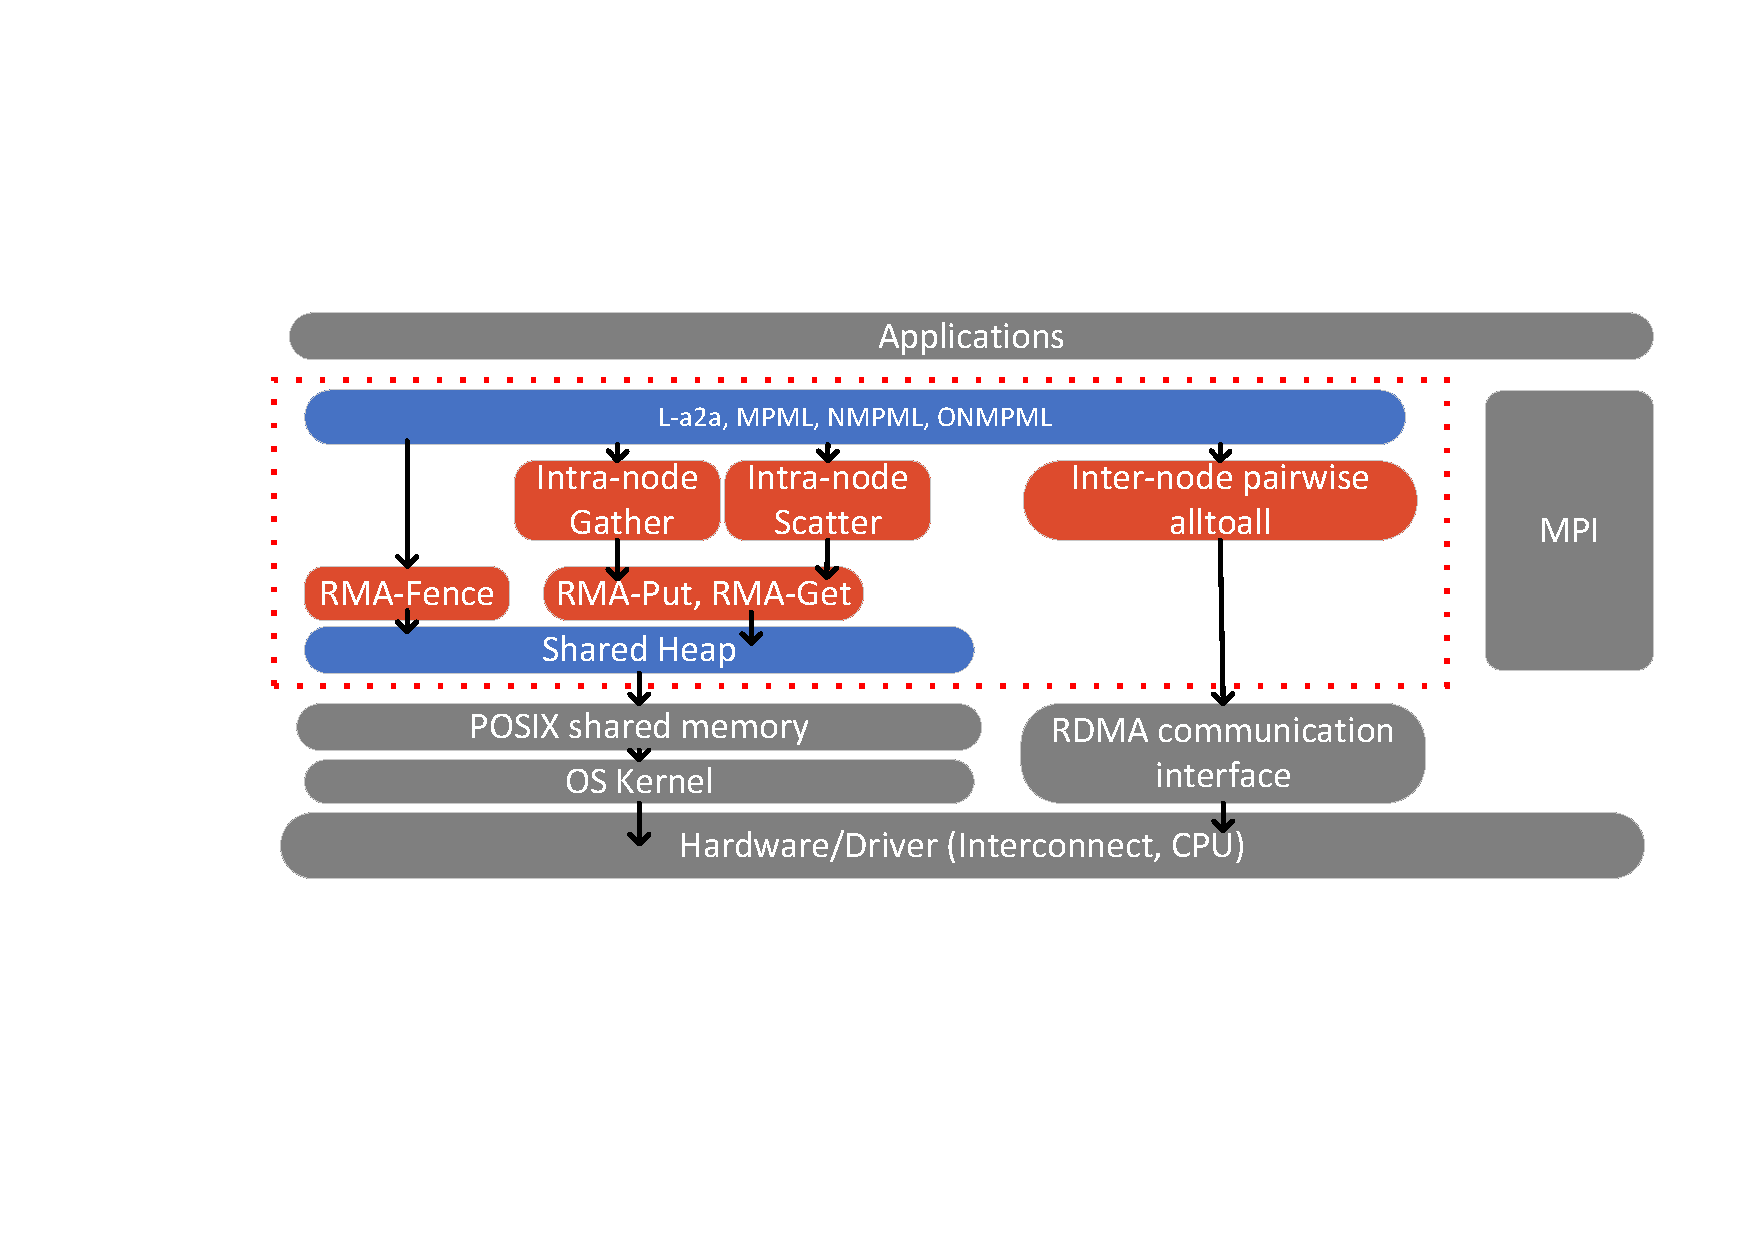
\includegraphics[width=16cm]{./Figures/implementaion.pdf} %[图片大小]{图片路径}
    \caption{Implementation overview.} %图片标题
    \label{fig:Implementation}
    \end{figure*}


As shown in Figure ~\ref{fig:Implementation}, the dash box include our impementation parts.
Our implemtation is based on shared memory and Galaxy Express (GLEX) communication layer (to support RDMA) for Tianhe series network.

\subsection {Impementation of Intra-node Communication}
Shared Heap \cite{friedley2013hybrid} is a large free shared memory  created by POSIX interface.
Then, each processes in a node associative the shared memory into its own addres space.
After that, a reimplented malloc (glex-malloc) which allocated the memory on this shared memory.
The memory allocated by glex-malloc are accessable by all ranks in a same node.
User's application must using glex-malloc to allocate sendbuf and recvbuf of all-to-all communication.
As a result, each processes in the node, can directly access the memory allocate on shared heap.

There is a set of intra-node operations RMA-fence, RMA-Put,and RMA-Get which based on shared heap. 
They are similar to MPI-Win-fence, MPI-Put and MPI-Get.
RMA-fence is a intra-node fence.
Between two RMA-fence, all ranks in a node is free to access other ranks buffer with RMD-Put and RMA-Get.
Difference is that a rank call RMA-Put or RMA-Get is blocking communication.
When  RMA-Put or RMA-Get return, the data is actually moved from one rank to another rank.


\subsection {Impementation of Inter-node Communication}

In gather-scatter-based all-to-all, the messages are aggregated. 
For most cases, they are large message.
In MPI, there are  eager protocol for small message and rendezvous protocol for large message.
Rendenzvous protocal have a "rendenzvous start" and "rendenzvous fin" overhead for each large message sending.
To avoid these protocal overhead, we directly use Remote Direct Memory Access (RDMA) to do inter-node communication.
RDMA communication must based on preregisted buffer.
This paper using two pre-registered buffer (BufferSend, BufferRecv) on each node to do inter-node RDMA.
Gathering operation direct gather the data on to BufferSend, than start RDMA communication. 
After receiver rank detect a receive event, it transpose the data and directly scatter the data on to receive buffer.
RDMA-based communication do not need  "rendenzvous start" and "rendenzvous fin" overhead for each large message transmission.
This avoids the overhead caused by the rendenzvous protocol.
\section{Evaluation}

\subsection{Microbenchmark Evalutation}
This paper evaluate performance of different based on following microbenchmark \ref{RDMASa2a}.

\begin{figure*}[!htb]
  \centering
    \subfigure[HPC-A:MPML compared to L-a2a]{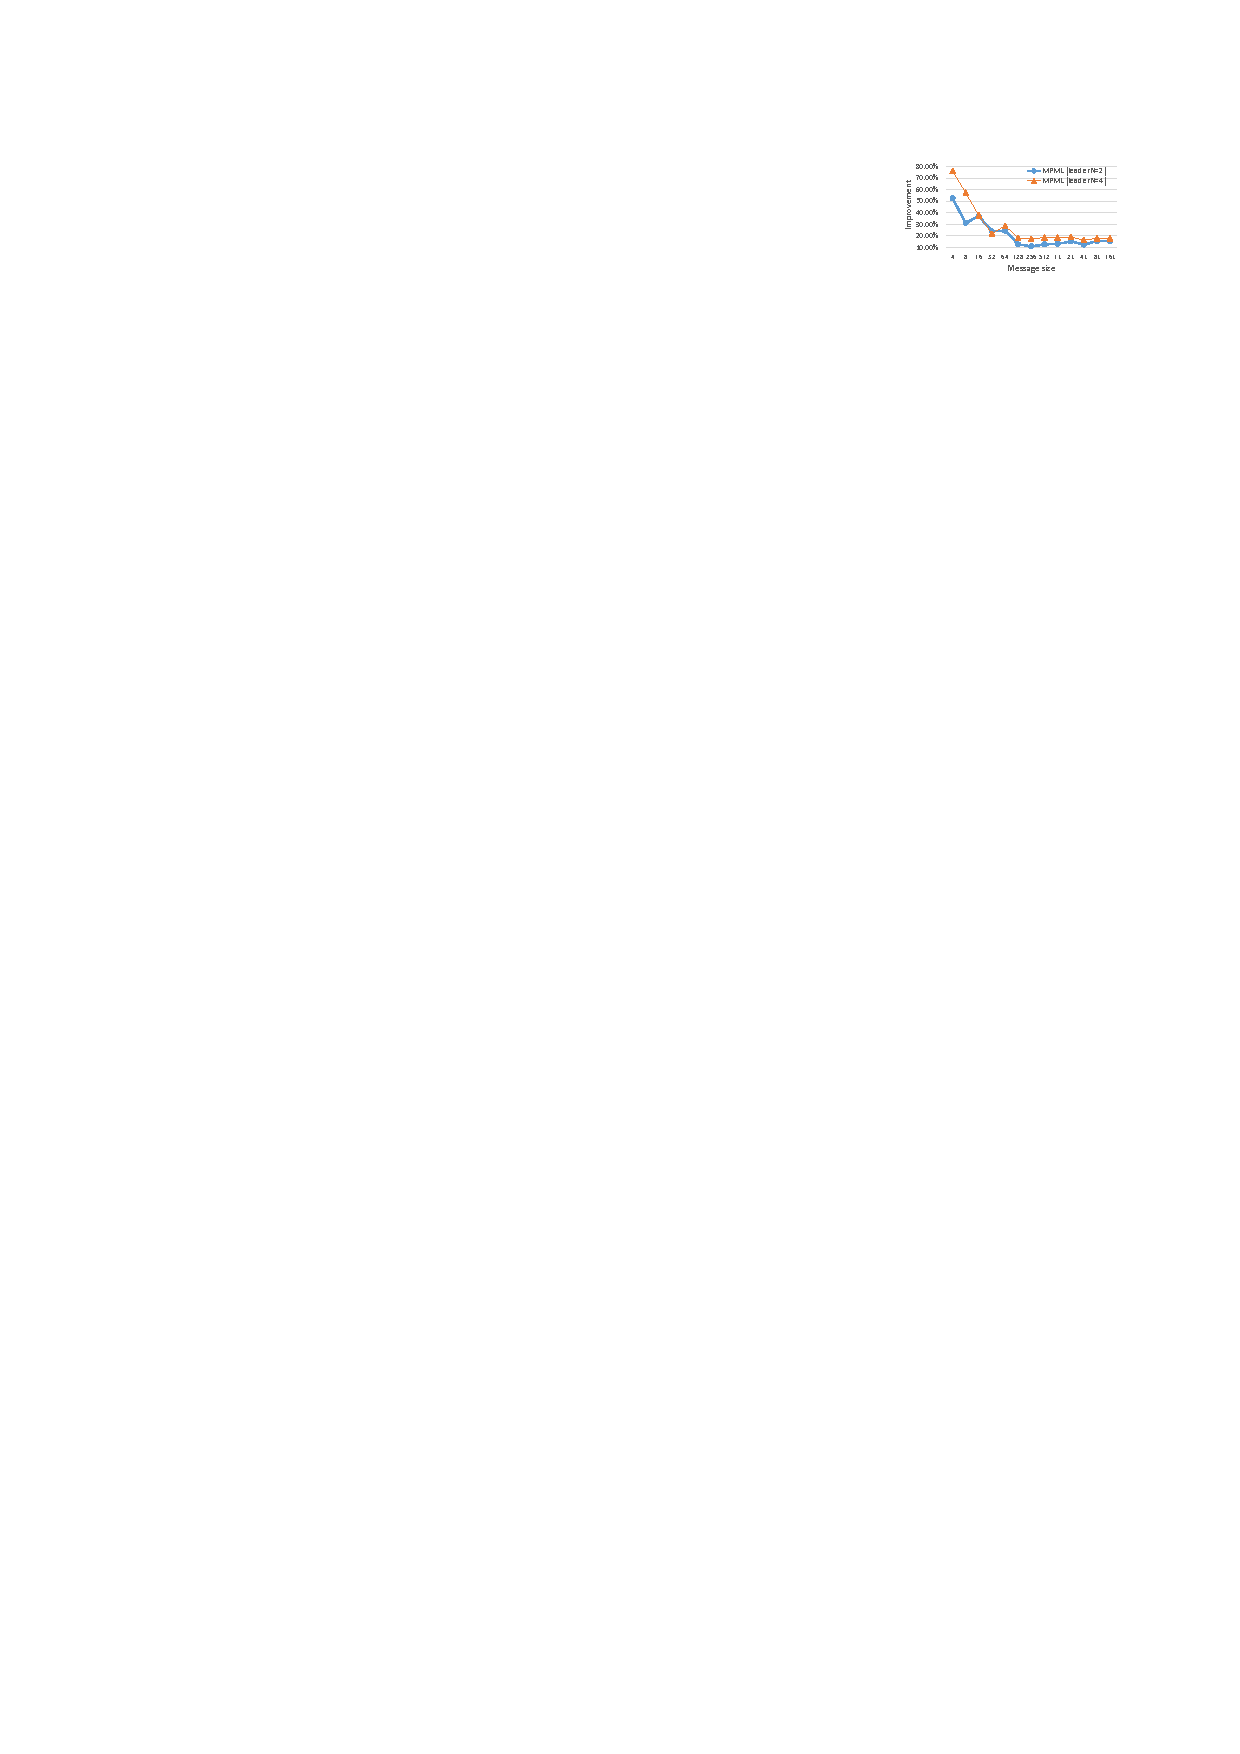
\includegraphics[width=0.45\textwidth]{./Figures/hpca/MPML.pdf}}
	\subfigure[HPC-A:NMPML compared to MPML]{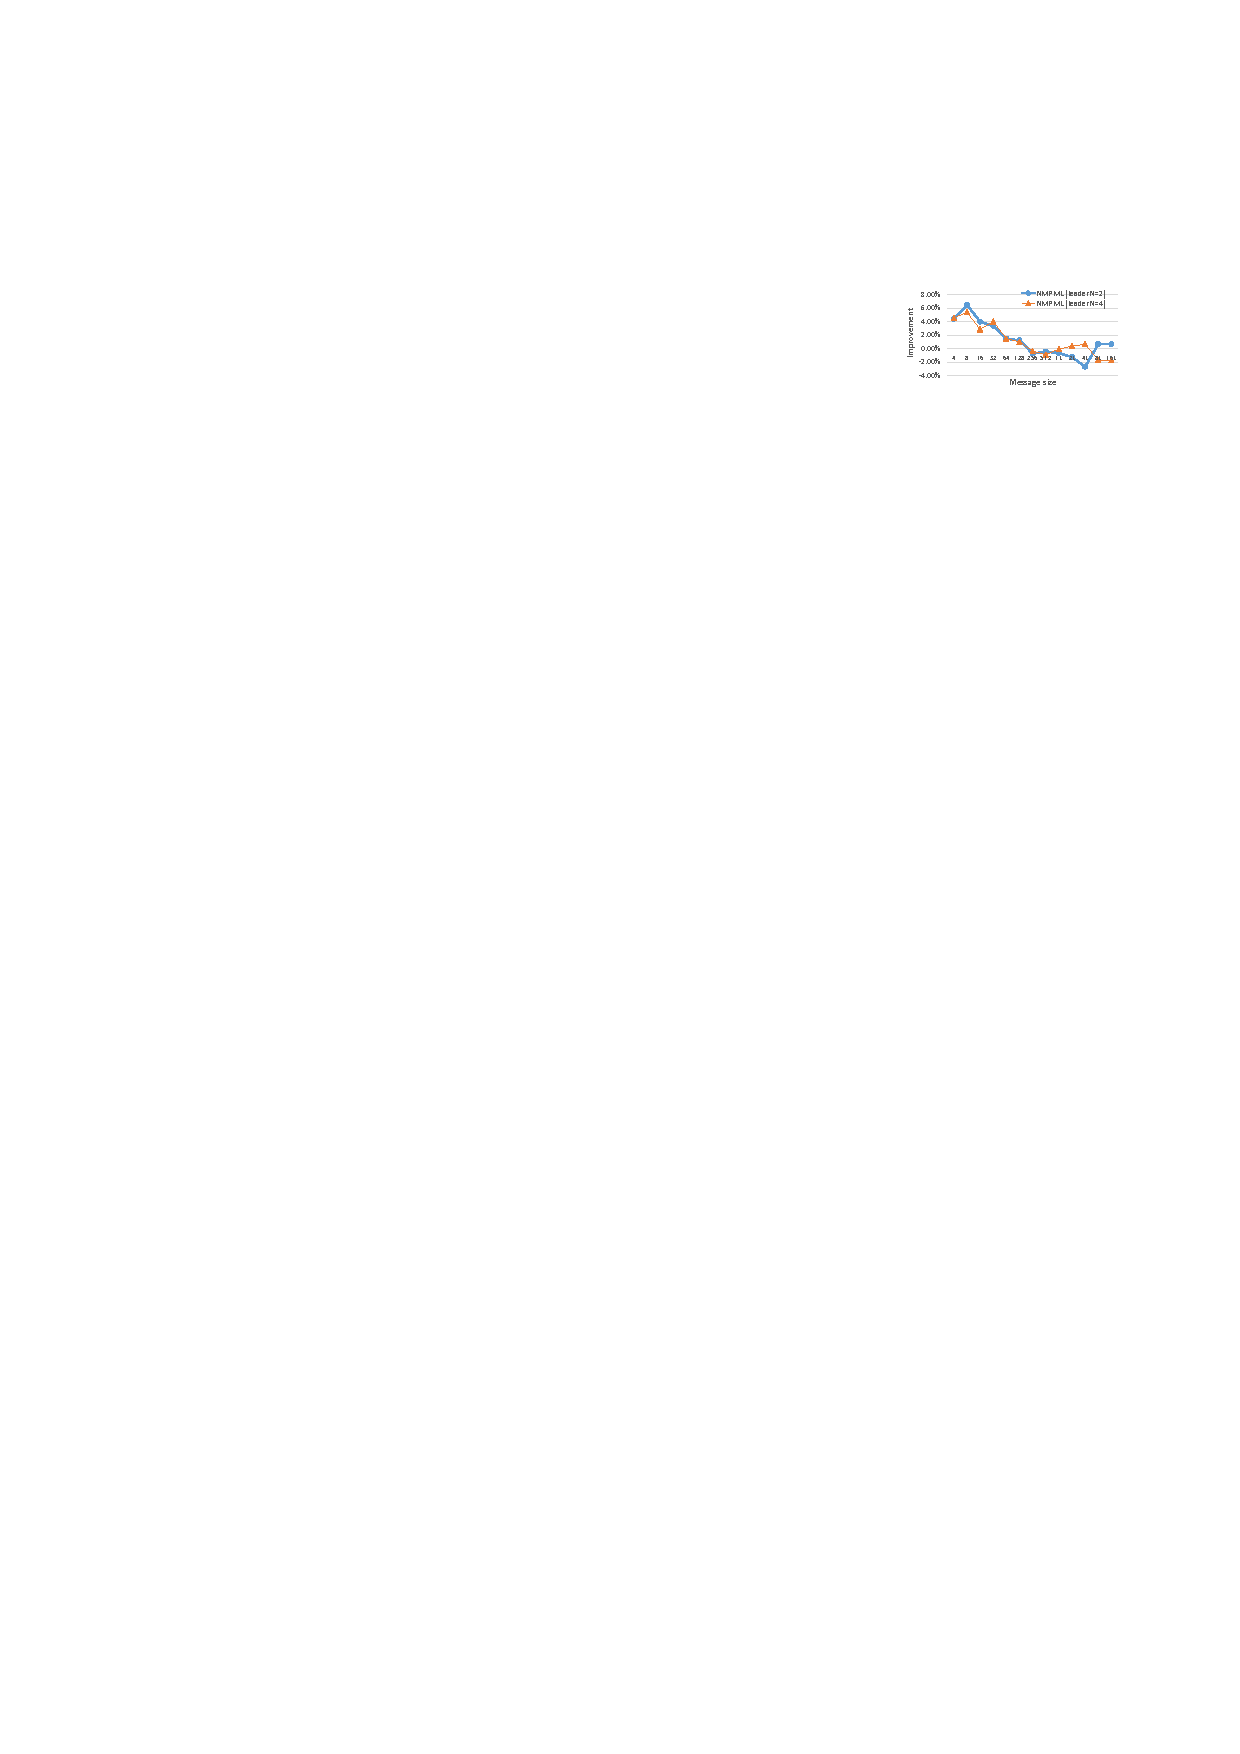
\includegraphics[width=0.45\textwidth]{./Figures/hpca/NMPML.pdf}}


    \subfigure[HPC-A:ONMPML compared to NMPML]{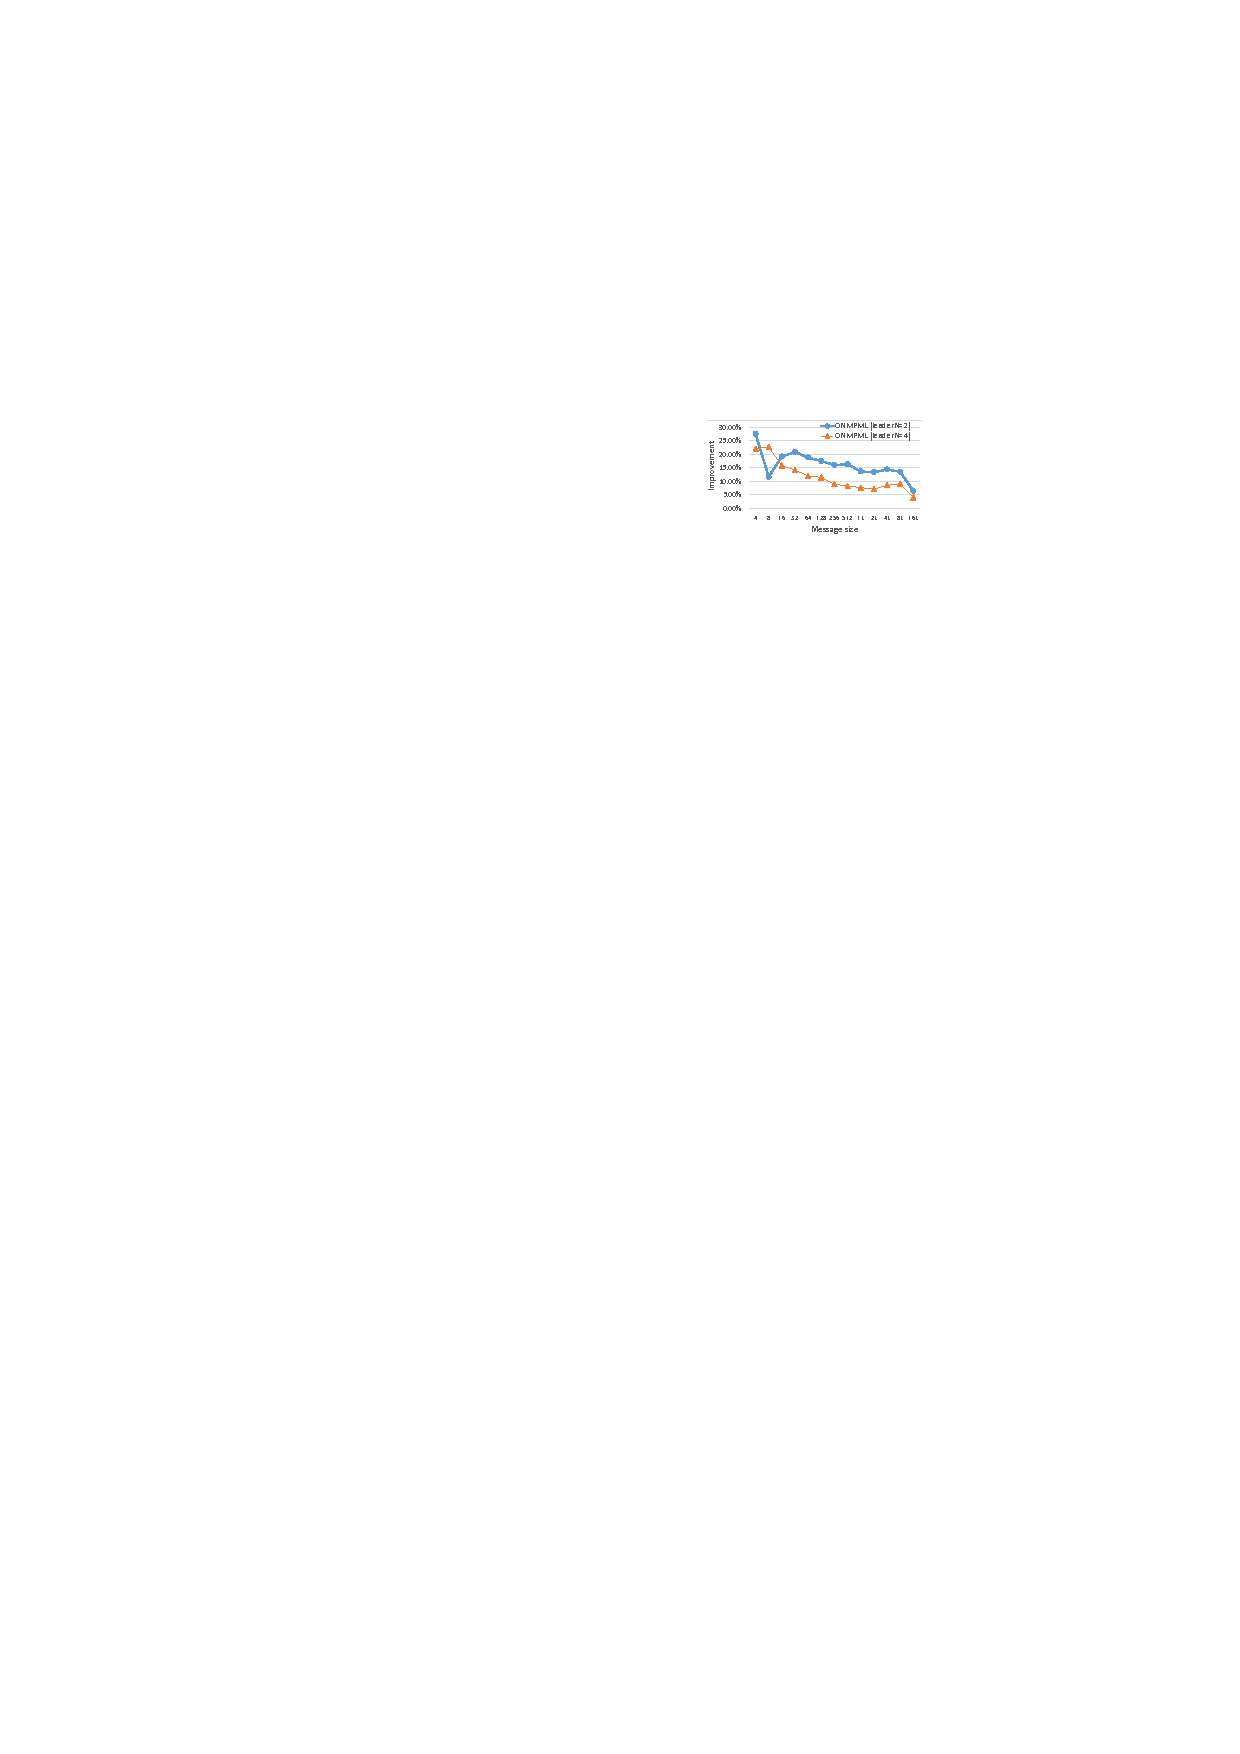
\includegraphics[width=0.45\textwidth]{./Figures/hpca/ONMPML.pdf}}
	\subfigure[HPC-A:ONMPML compared to MPI]{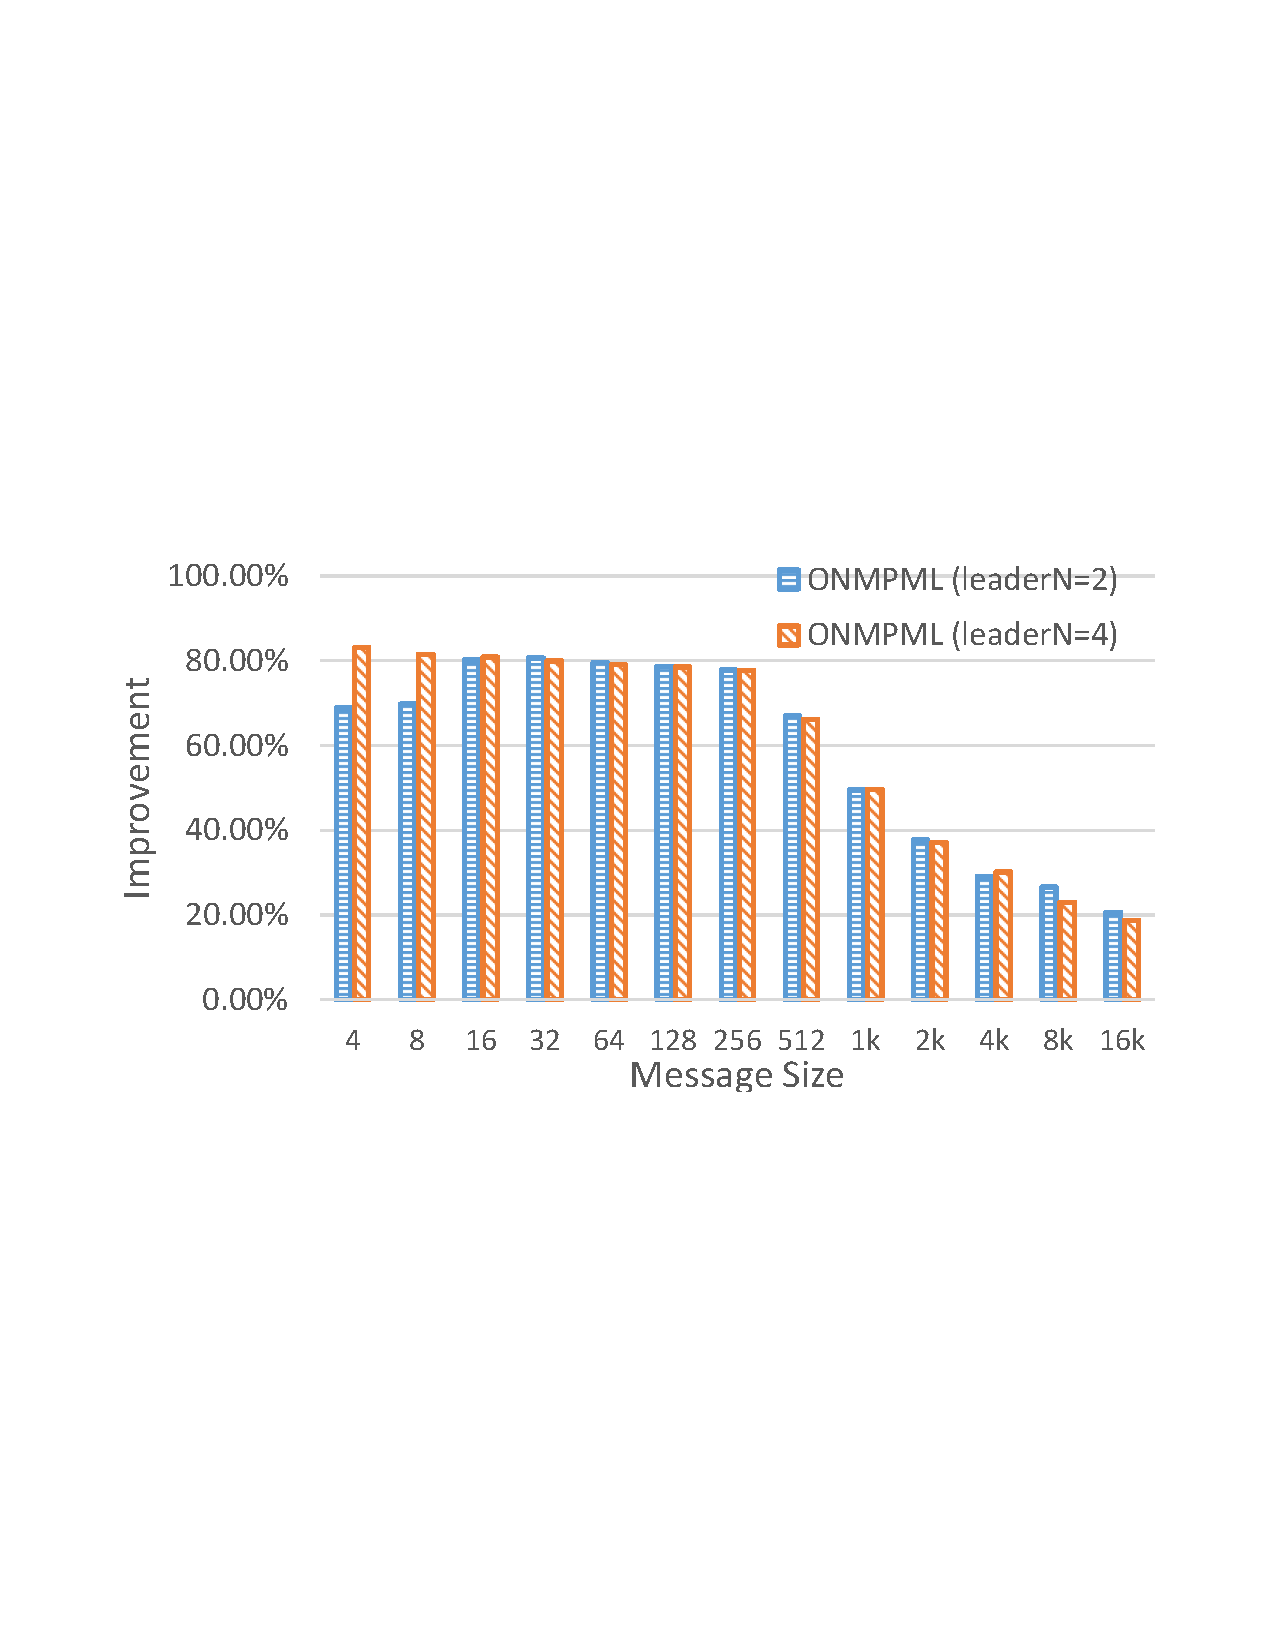
\includegraphics[width=0.45\textwidth]{./Figures/hpca/ONMPML-MPI.pdf}}
  \caption{Microbenchmark results of 256 nodes, 8192 processes alltoall collective on HPC-A.}
	\label{HPCA-EXPR}
	\vspace{0.2in}
\end{figure*}

\begin{algorithm}
\caption{all-to-all microbenchmark}\label{RDMASa2a}
{
	\For{ i in range(0,loopN)}
	{
		MPI\_Barrier(comm) \\
		startT = MPI\_Wtime() \\
		Alltoall() \\
		endT = MPI\_Wtime() \\
		totalT += (endT-start)
	}
	MPI\_Reduce(totalT,MaxT) \\
	MaxT $\leftarrow \frac{MaxT}{loopN}$ 
}
It compares the MPI\_Alltoall to our RDMA-based Alltoall (L-a2a, MPML, NMPML, ONMPML) on different HPC systems.
\end{algorithm}
\subsubsection{Microbenchmark Result on HPC-A}
The results of microbenchmark on four HPC systems are shown in Figure ~\ref{HPCA-EXPR}.
We can see that multi-endpoint, multi-leader alltoall (MPML) has a better performance than one leader alltoall (L-a2a).
When we using 4 leaders, its faster than 2 leader MPML.
In subfigure a of Figure \ref{HPCA-EXPR}, the improvement going down as the message getting larger.
As the HPC-A has the 1.3 GB/s bidirectional network bandwidth among these systems, which is far slower than the gatering/scattering bandwidth.
The whole alltoall is limited by the network bandwidth for large message.
As a result, MPML has a lesser performance improvement on a low-bandiwidth, large message alltoall.

Subfigure b of Figure \ref{HPCA-EXPR} show the performance of NUMA-aware MPML compared to MPML.
2-leader NMPML is compared to 2-leader MPML. 4-leader NMPML is the same the 2-leader NMPML.
For small message NUMA-aware MPML has a little performance improvement compared to MPML.
The large message has nearly no improvement.
This is same with the Figure \ref{UMA-aware-multi-leader}. The NUMA-aware gathering-scattering has batter throughput on small messages.

Subfigure c of Figure \ref{HPCA-EXPR} show that the ONMPML compared to corresponding NMPML.
ONMPML has a significant performance improvement. 
As ONMPML overlaped the inter-node and intra-node communication.
Subfigure d show the ONMPML compared to MPI\_Alltoall on HPC-A.
4-leader ONMPML has a 3.53x  speedup  on average compared to MPI\_Alltoall.
\subsubsection{Microbenchmark Result on HPC-B}
\begin{figure*}[!htb]
  \centering
    \subfigure[HPC-B:MPML compared to L-a2a]{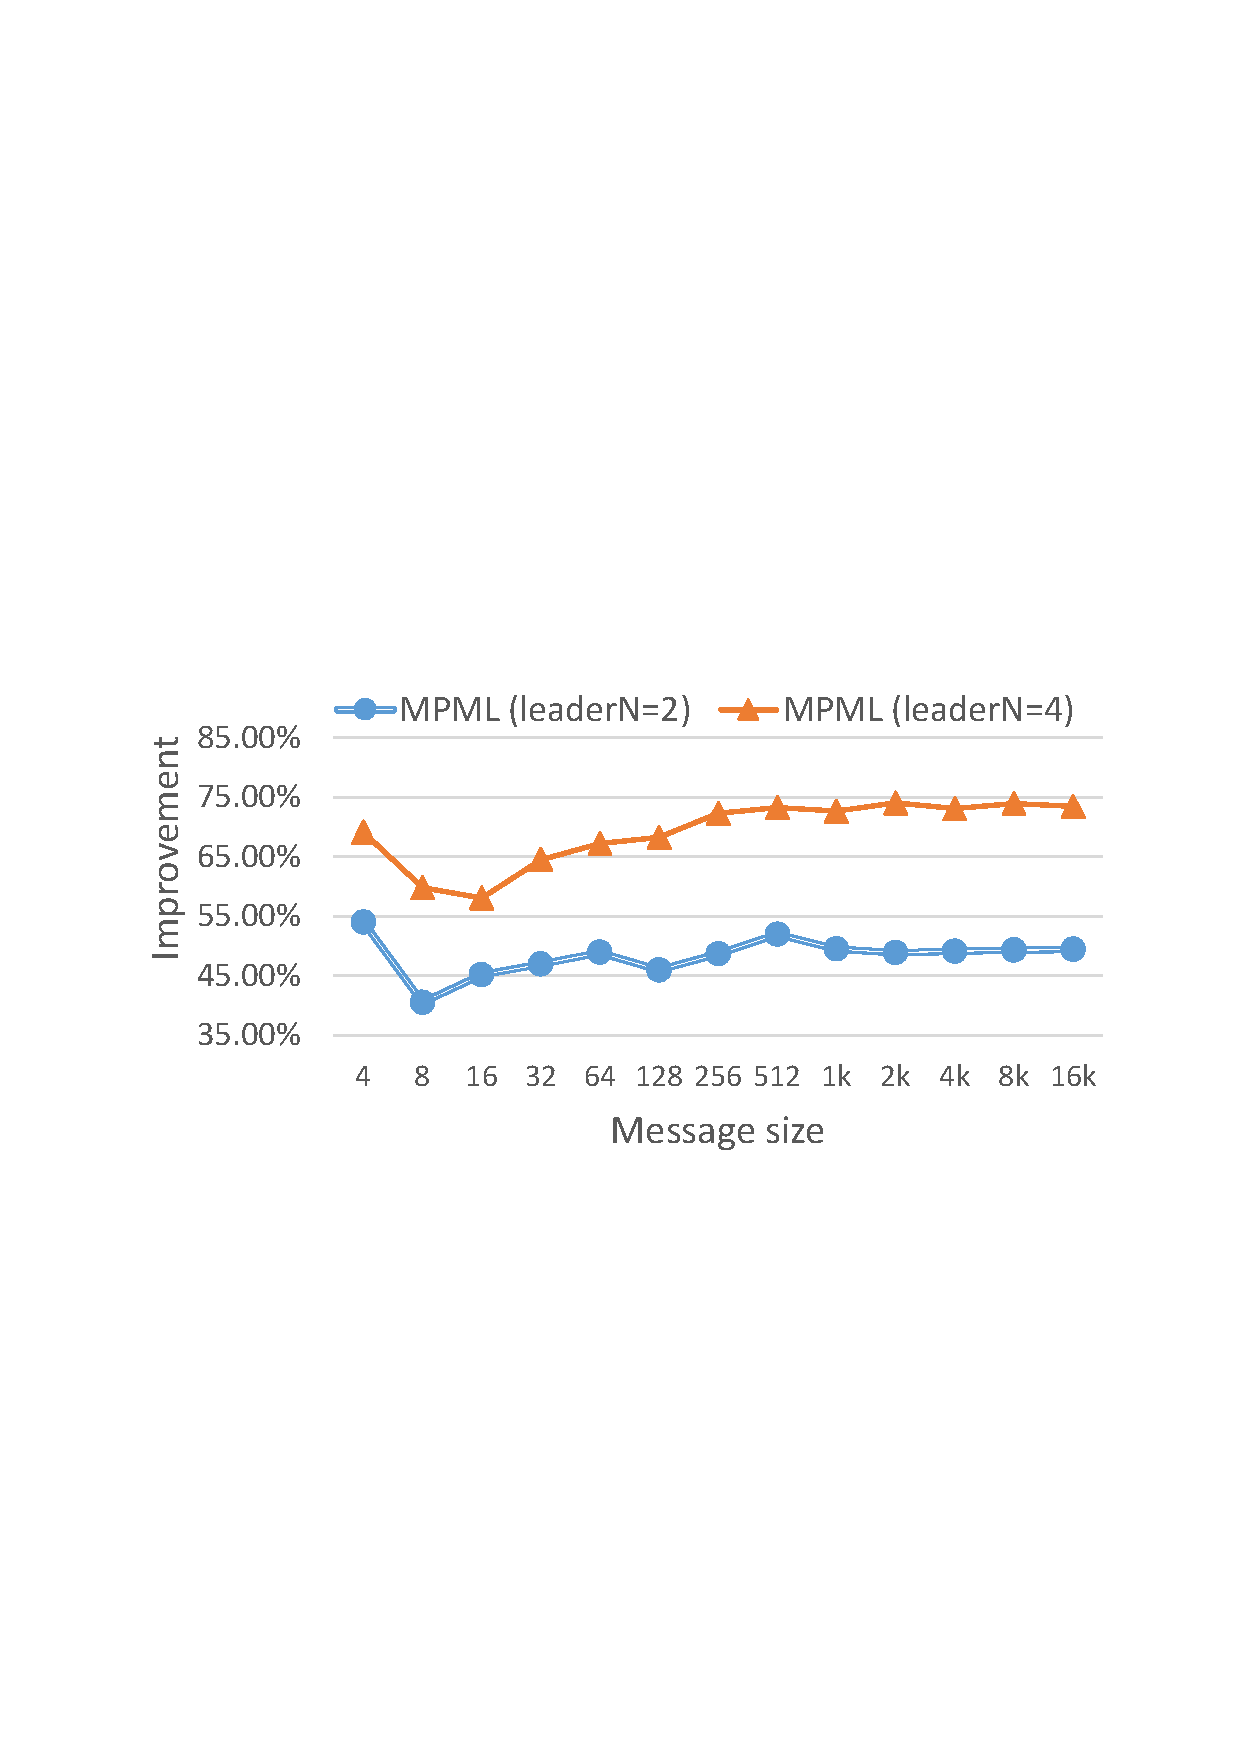
\includegraphics[width=0.45\textwidth]{./Figures/hpcd/MPML.pdf}}
	\subfigure[HPC-B:NMPML compared to MPML]{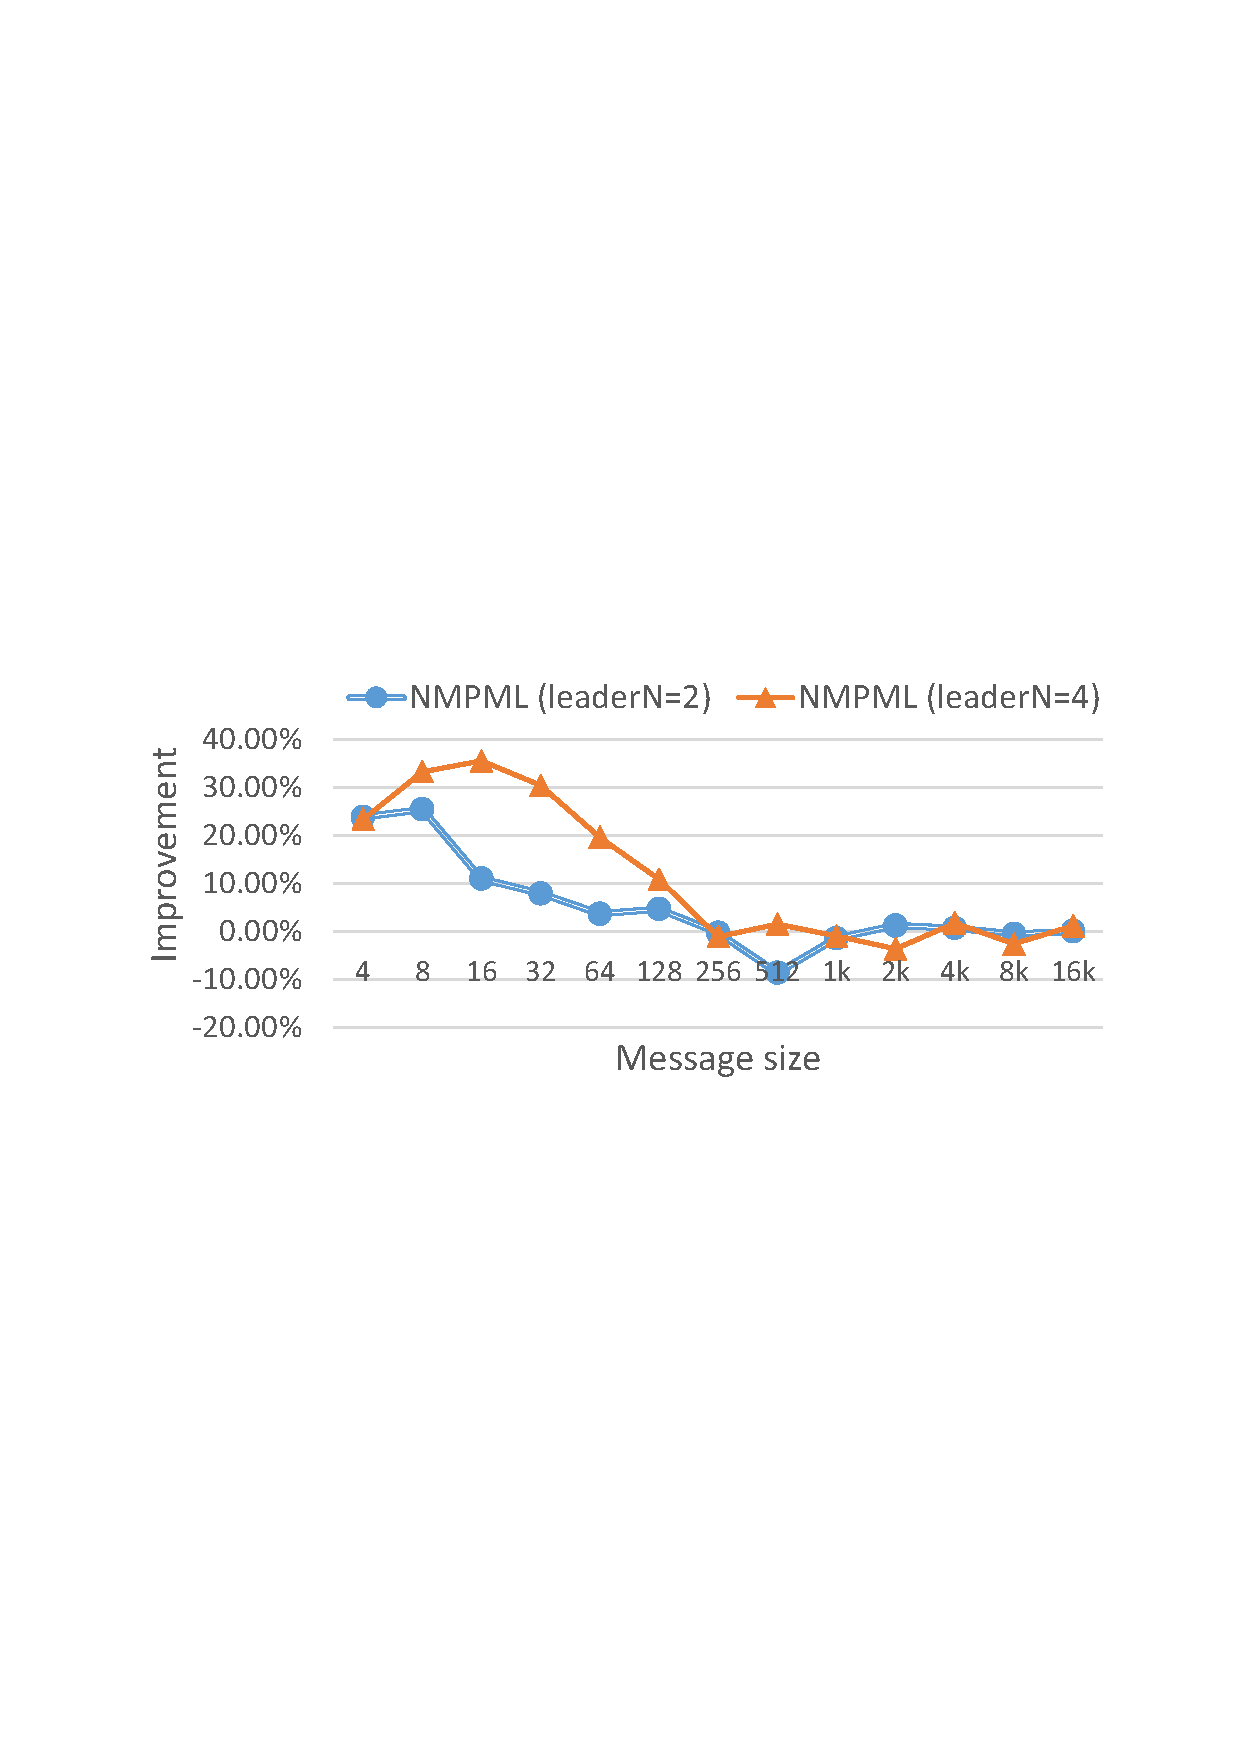
\includegraphics[width=0.45\textwidth]{./Figures/hpcd/NMPML.pdf}}


    \subfigure[HPC-B:ONMPML compared to NMPML]{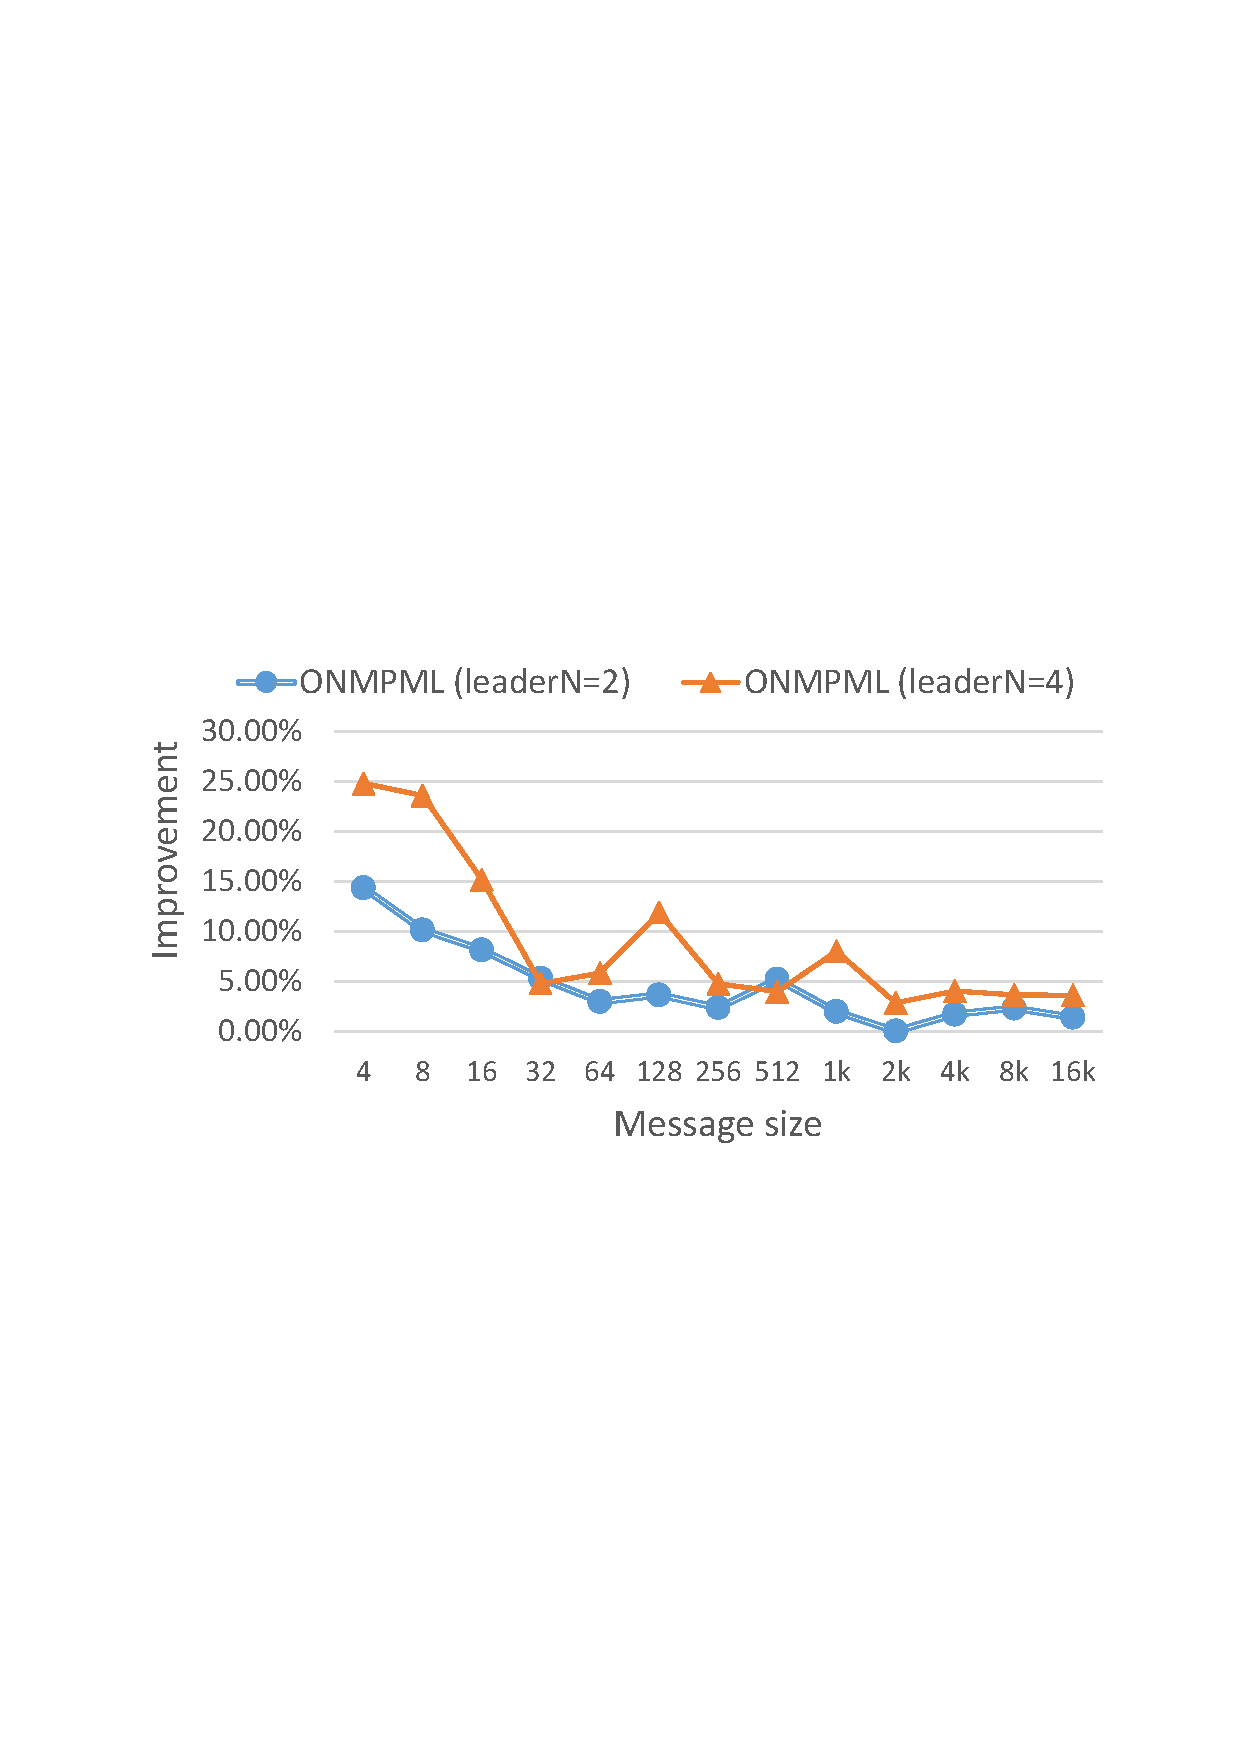
\includegraphics[width=0.45\textwidth]{./Figures/hpcd/ONMPML.pdf}}
	\subfigure[HPC-B:ONMPML compared to MPI]{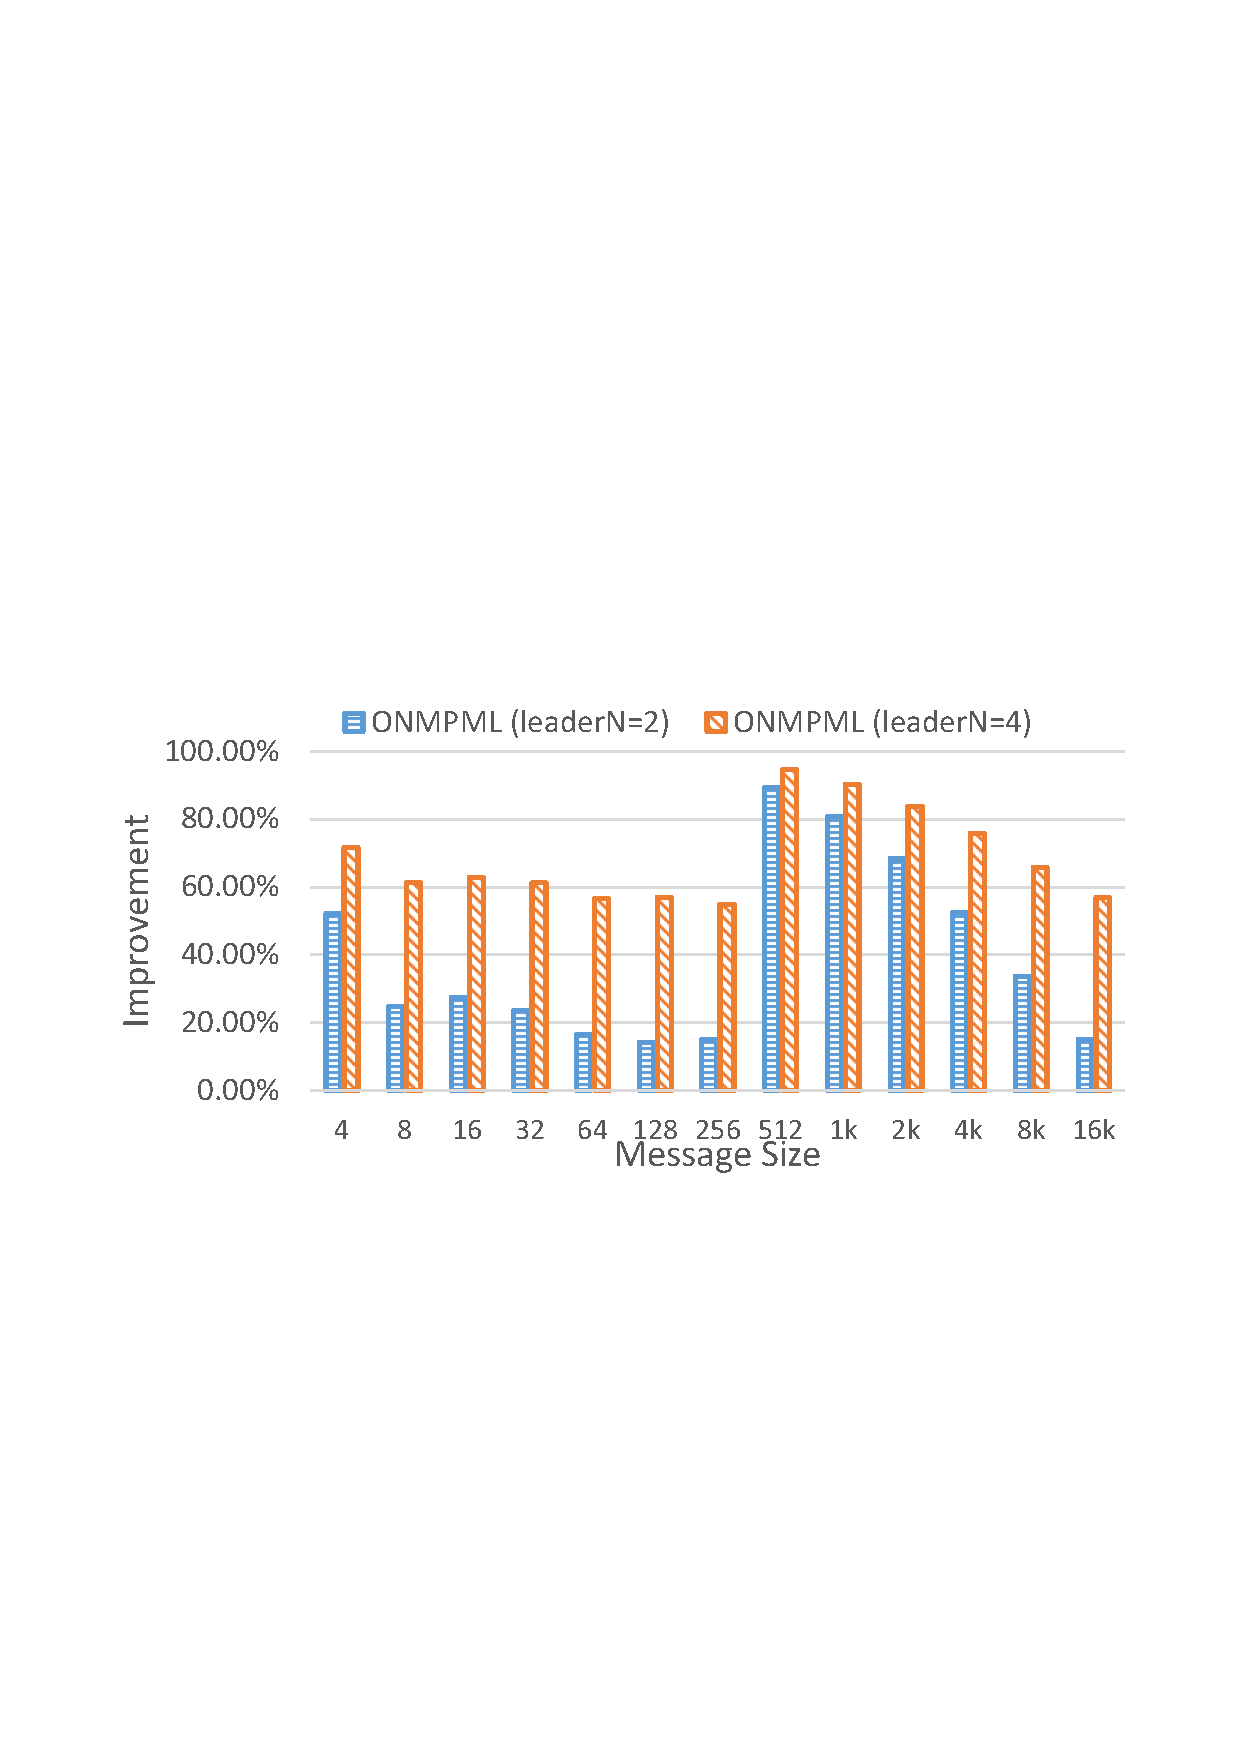
\includegraphics[width=0.45\textwidth]{./Figures/hpcd/ONMPML-MPI.pdf}}
  \caption{Microbenchmark results of 50 nodes, 1200 processes alltoall collective on HPC-B.}
	\label{HPCD-EXPR}
	\vspace{0.1in}
\end{figure*}
For subfigure a of Figure \ref{HPCD-EXPR}, MPML show a 45\% or 65\% improvement compared to L-a2a. This is because its bisectional network bandwidth is 11 GB/s. one leader's gathering/scattering throughput are 6 GB/s. The intra-node communication may take up a major part of communication overhead. As a result, MPML can obliviously improve the performance compare to L-a2a under the big messages.

For subfigure b of Figure \ref{HPCD-EXPR}, NMPML still show a little performance improvement for small messages.
Subfigure c show that 5\%(2-leader ONMPML) and 12.5\%(4-leader ONMPML) performance improvement compared to NMPML.
Compare to MPI\_Alltoall, 4-leader ONMPML acheives 3.7x speedup on average.

\subsection{HPCC-FFT Evaluation}
HPC Challenge is a benchmark suite which combines several benchmarks to test the performance of high-performance computer (HPC) systems \cite{luszczek2006hpc}.
Their is a global Fast Fourier Transforms (FFT) benchmark in HPCC.
FFT is very useful in applications such as spectral methods, signal processing and climate modeling.
HPCC global FFT doing a 1D FFT Z=FFT(X). 
MPI\_Alltoall is used to transpose matrix in global FFT.
We replace the MPI\_Alltoall with our 4-leader ONMPML based on GLEX RDMA (GLEX\_Alltoall).
We stested different vector size Ns. For HPC-A we test Ns=\{256,512,1024,2048\}.
For HPC-B, we test Ns=\{512,1024,2048,4096\}.
The result shown as Figure \~ref{App-EXPR}.
\begin{figure*}[!htb]
  \centering
    \subfigure[HPC-A: 256 nodes]{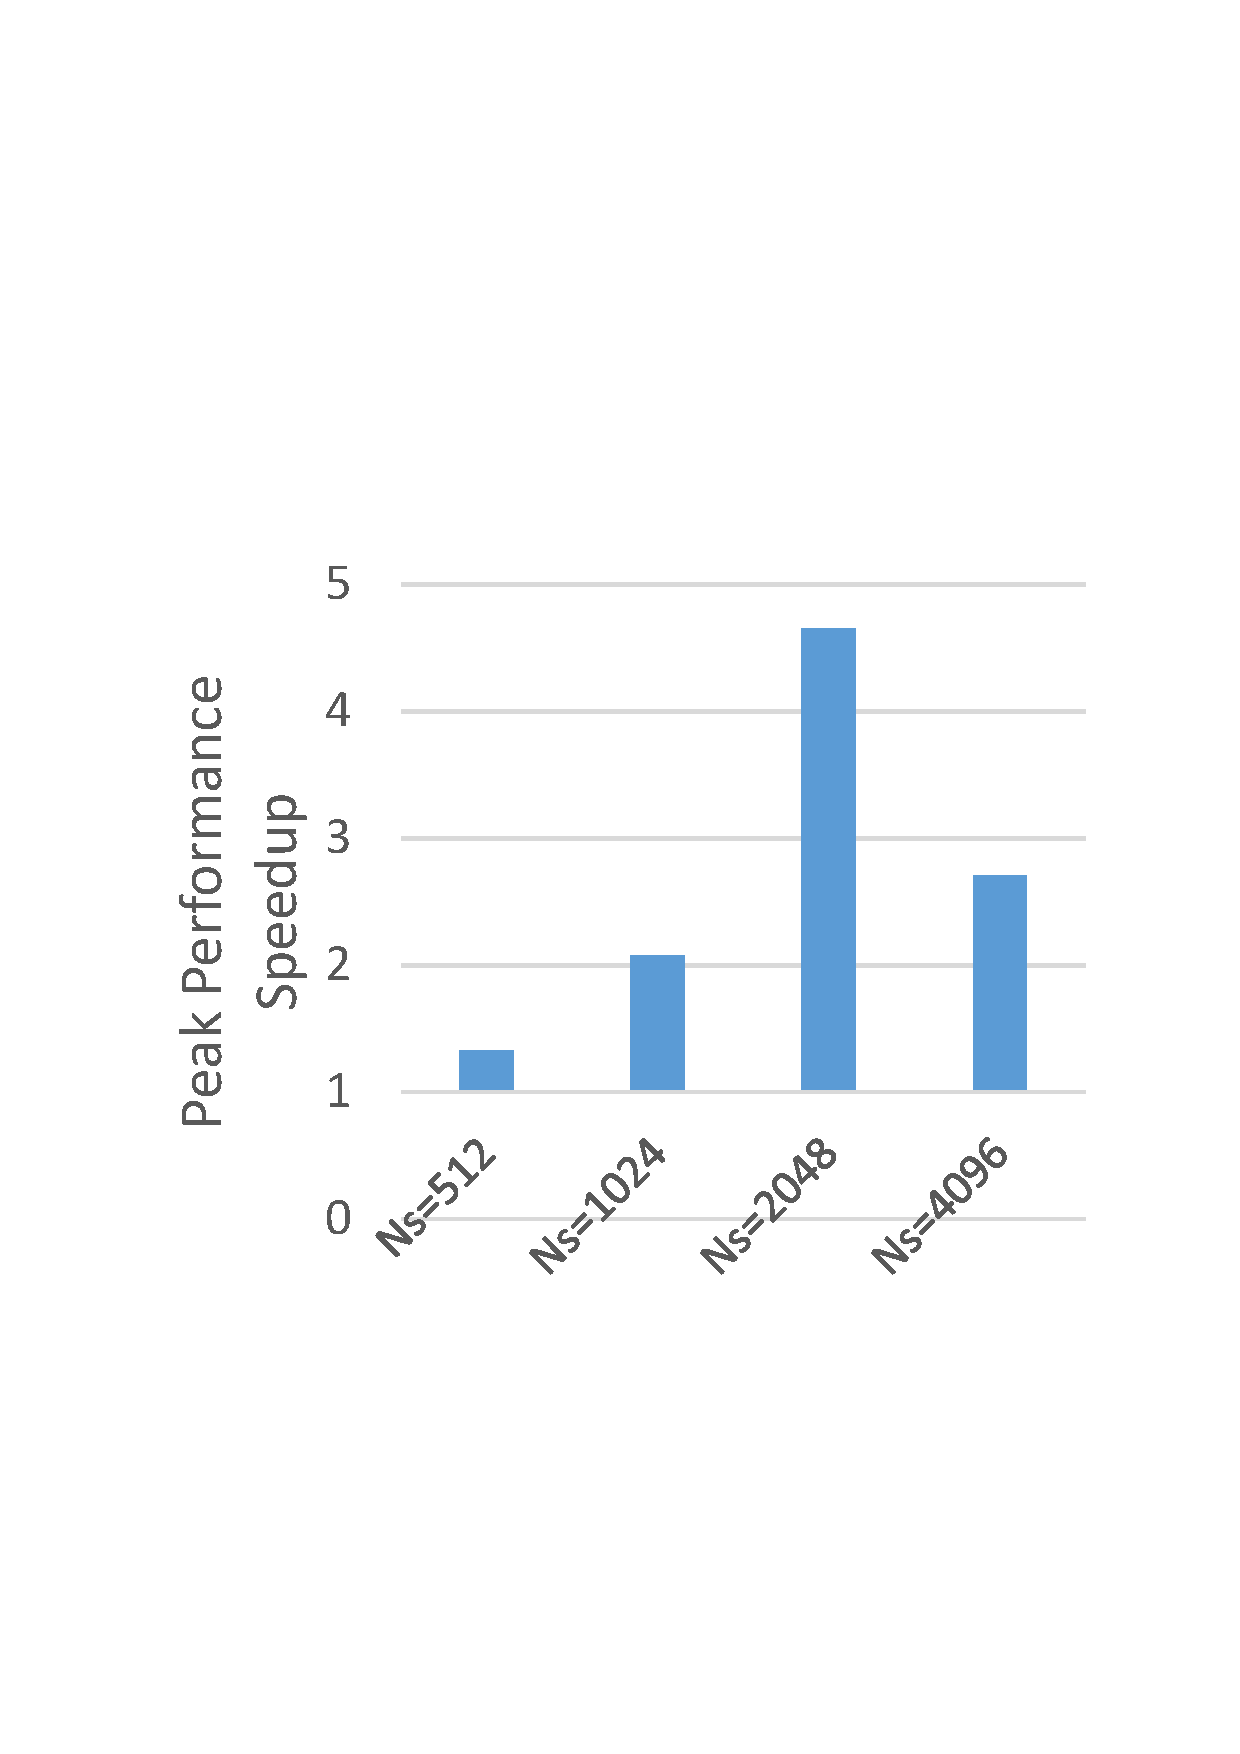
\includegraphics[width=0.32\textwidth]{./Figures/hpca/FFT.pdf}}
	\subfigure[HPC-B: 200 nodes]{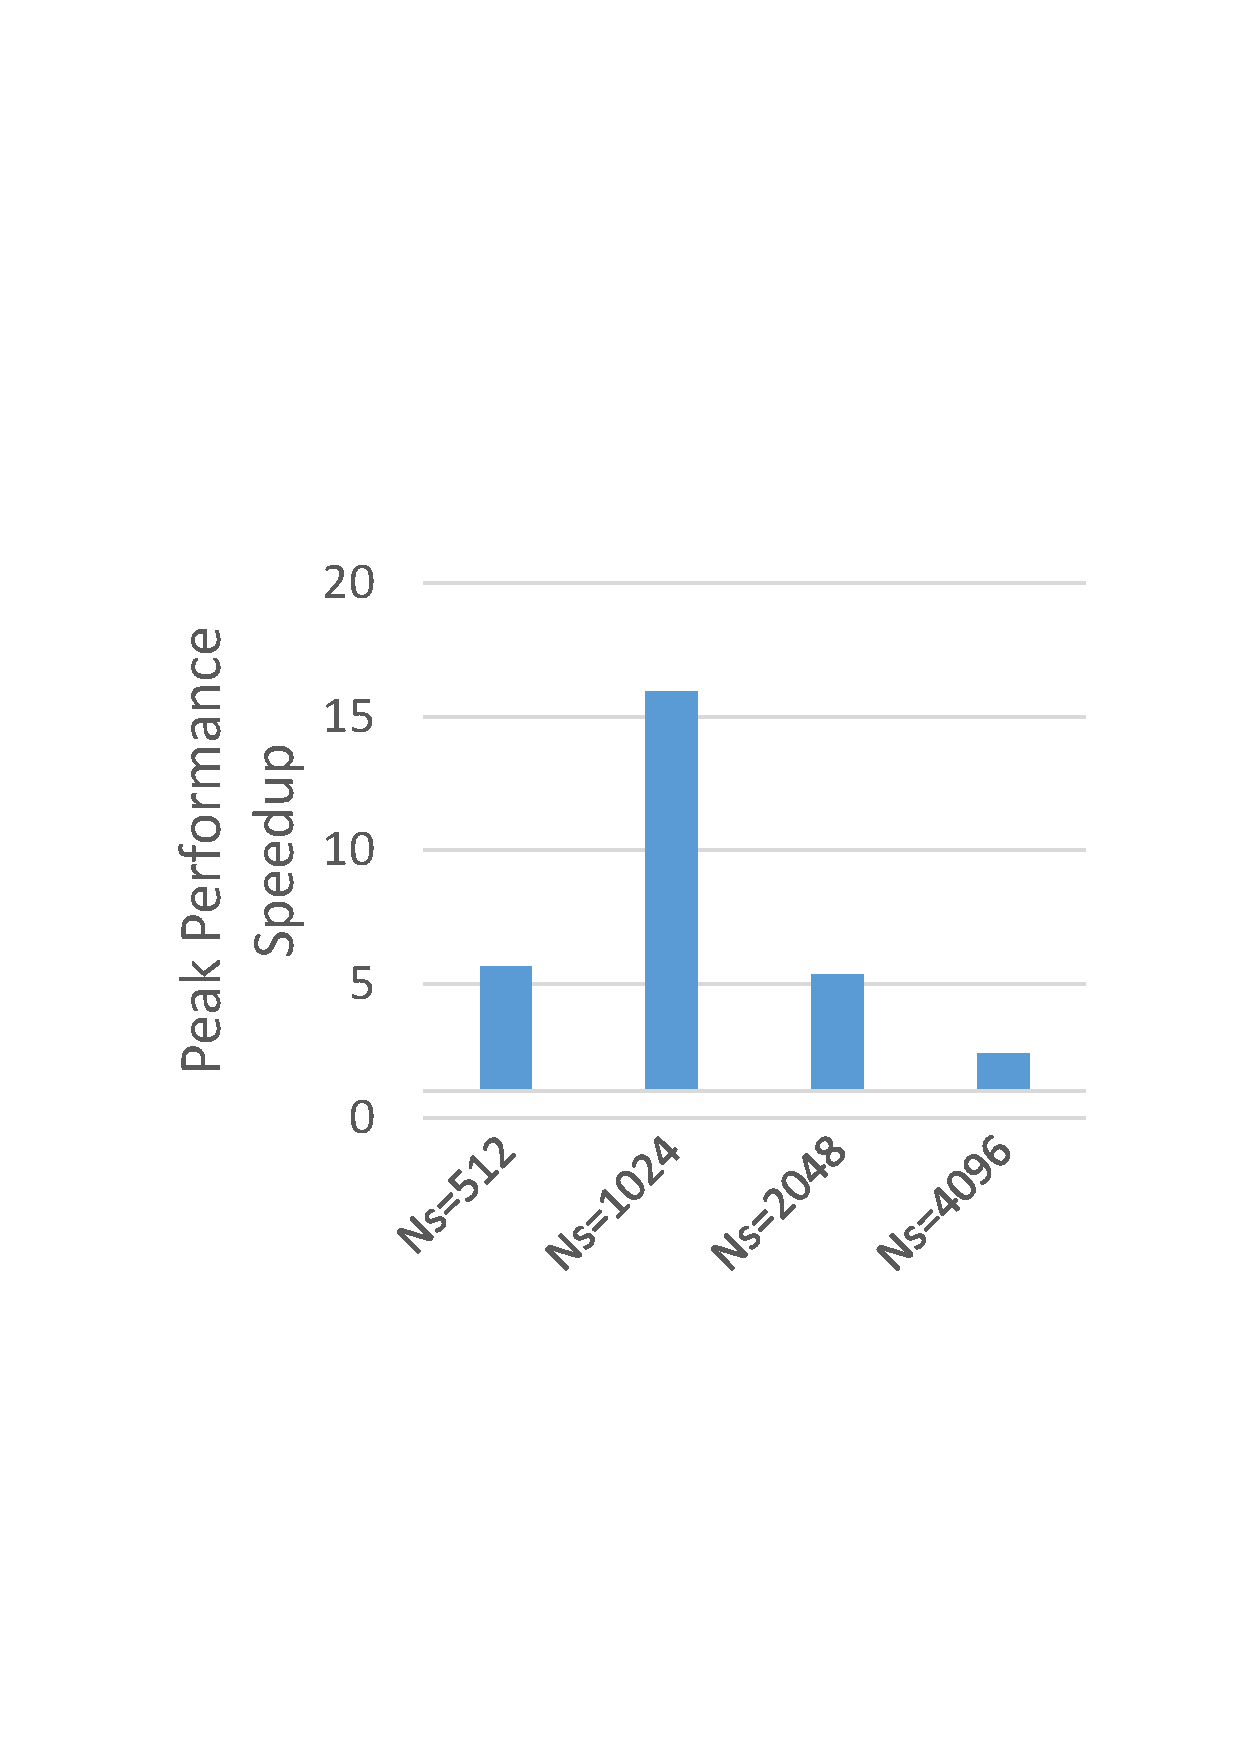
\includegraphics[width=0.32\textwidth]{./Figures/hpcd/FFT.pdf}}
  \caption{Application evaluations.}
	\label{App-EXPR}
	\vspace{0.1in}
\end{figure*}



\bibliography{mybibfile}

\end{document}